\documentclass[11pt]{article}
\usepackage[a4paper,margin=1in]{geometry}
\usepackage{amsmath,amssymb,amsfonts}
\usepackage{booktabs}
\usepackage{graphicx}
\usepackage{caption}
\usepackage{enumitem}
\usepackage[table]{xcolor}
\usepackage{array}
\usepackage[hidelinks]{hyperref}
\usepackage{xurl}
\usepackage{microtype}

\title{2D One-/Two-Target Gating Mechanism Report\\\large one-target reset to a shared symmetric baseline with balanced asymmetric comparisons}
\author{}
\date{}

\setlist{nosep}
\setlength{\textfloatsep}{8pt plus 2pt minus 2pt}
\setlength{\floatsep}{6pt plus 2pt minus 2pt}
\setlength{\intextsep}{6pt plus 2pt minus 2pt}
\setlength{\abovecaptionskip}{4pt}
\setlength{\belowcaptionskip}{0pt}
\setlength{\tabcolsep}{5pt}
\renewcommand{\arraystretch}{1.10}

\begin{document}
\maketitle

\section*{Headline Result}
This report still preserves the March 16 source chain
\texttt{membrane\_gating\_game}
$\rightarrow$
\texttt{two\_target\_gating\_framework}
$\rightarrow$
\texttt{one\_two\_target\_deepening\_work},
but the one-target branch has now been reset onto a more stable configuration logic:
\begin{itemize}
  \item the \textbf{standard configuration} is the shared symmetric baseline \texttt{sym\_shared}, not an extreme asymmetric point;
  \item the manuscript separates two distinct notions of asymmetry: \textbf{top/bottom membrane asymmetry} and \textbf{same-membrane directional asymmetry};
  \item \textbf{rollback} is retained as the main one-target discrete mechanism, but now in a \emph{gate-free} form: after leaving the start basin $A$, does the trajectory later re-enter $A$;
  \item the real-set \textbf{x-gate} remains, but only as a time-anchor line for the $N/P/Q$ mechanism;
  \item \textbf{loss of bimodality} is defined strictly as \texttt{phase=0}; \texttt{phase=1} means weakening, not disappearance of the second peak.
\end{itemize}

\section{Source Chain and Current Role}
\paragraph{Why the one-target branch needed to be rewritten again.}
The previous canonical integration had already absorbed the 6 downloaded files into shared code and a standard report layout, but the one-target main language was still not stable enough: extreme $\kappa=0$ points were too exhibition-like, and rollback remained too tightly tied to the $x=X_g$ gate. The present revision resets the one-target section to a more geometric and more repository-native language.

\begin{figure}[!htbp]
  \centering
  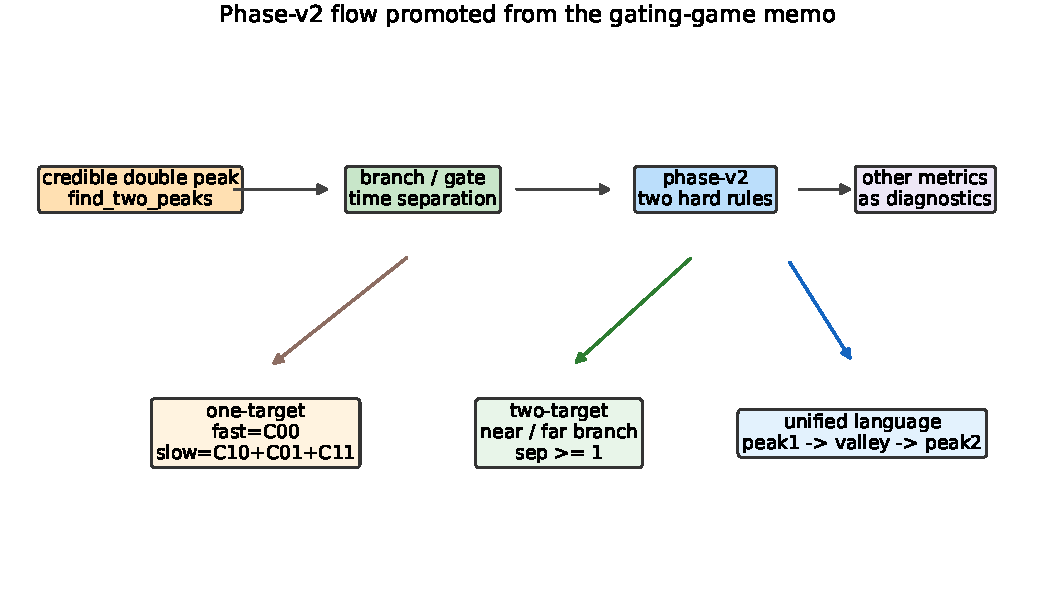
\includegraphics[width=0.84\linewidth]{../artifacts/figures/gating_game_phase_v2_flow.pdf}
  \caption{The phase-v2 / gating-game source sketch. The current canonical report keeps the source chain, but no longer lets the older gate language dominate the one-target main text.}
\end{figure}

\begin{figure}[!htbp]
  \centering
  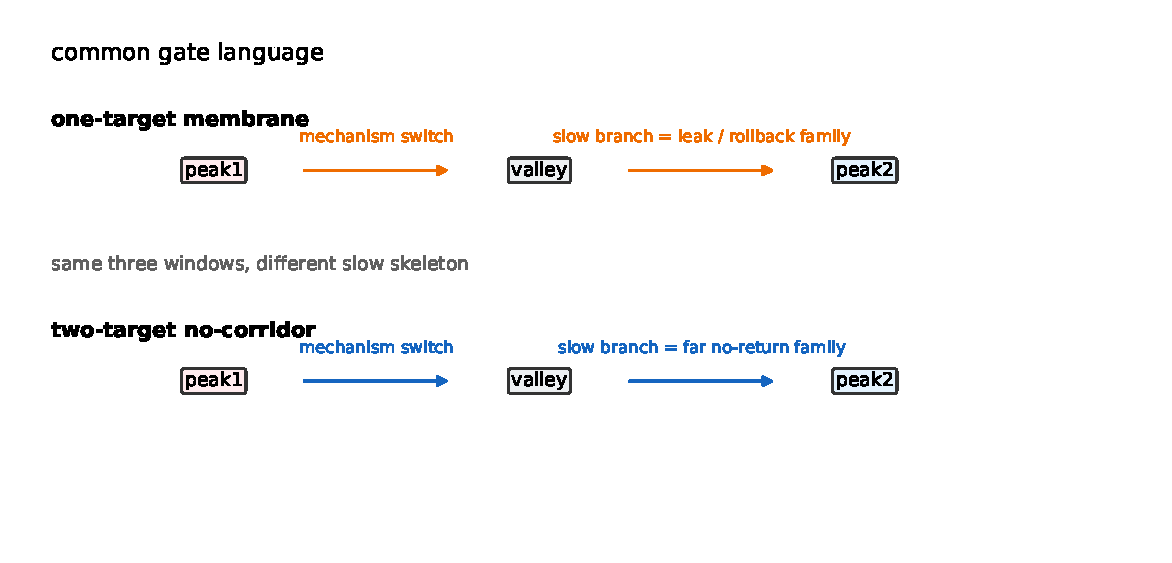
\includegraphics[width=0.92\linewidth]{../artifacts/figures/unified_mechanism_ladder.pdf}
  \caption{Unified mechanism ladder. The two-target branch still uses the gate-lifted family language, while the one-target branch is now organized around a shared symmetric baseline, gate-free rollback classes, and x-gate timing diagnostics.}
\end{figure}

\section{The one-target standard configuration and the two symmetries}
\paragraph{What the standard configuration is.}
The one-target standard configuration is now fixed as
\[
\texttt{sym\_shared}:\qquad
\kappa_{\rm top}=\kappa_{\rm bottom}=k_{\rm ref}=0.002,
\]
which simultaneously satisfies the directional symmetry condition
\[
\kappa_{c\to o}=\kappa_{o\to c}=0.002.
\]
So \texttt{sym\_shared} is the unique shared baseline for both symmetry notions.

\paragraph{Why the canonical representatives are no longer extreme.}
Extreme points remain useful as controls or phase-loss boundaries, but they are no longer used as the main representatives. The current representatives are selected by a fixed scan rule:
\begin{itemize}
  \item prefer \texttt{phase=2};
  \item prefer interior points with both parameters strictly positive;
  \item prefer points close to fixed balanced anchors, while still keeping strong peak separation;
  \item if the nominal anchor is not itself phase-2, select the nearest phase-2 interior point in the same directional class.
\end{itemize}
As a result, the non-symmetric representatives are now balanced comparison cases rather than ``one side completely shut'' showcase points.

\begin{table}[!htbp]
  \centering
  \caption{Canonical one-target representative cases. The table explicitly distinguishes the standard configuration from comparison configurations and records the actual parameters, phase, and separation values.}
  \begin{tabular}{lllrrllr}
\toprule
case & role & parameters & phase & sep & peak2 rollback & peak2 gate & rollback \\
\midrule
shared symmetric baseline & standard & $(\kappa_{c\to o},\kappa_{o\to c})=(0.0020,0.0020)$ & 2 & 1.528 & L0R1 & N & 89.2\% \\
top/bottom balanced asymmetry & comparison & $(\kappa_{top},\kappa_{bottom})=(0.0020,0.0005)$ & 2 & 1.689 & L0R1 & N & 89.1\% \\
directional easy-out / hard-return & comparison & $(\kappa_{c\to o},\kappa_{o\to c})=(0.0020,0.0005)$ & 2 & 1.614 & L0R1 & N & 89.3\% \\
directional hard-out / easy-return & comparison & $(\kappa_{c\to o},\kappa_{o\to c})=(0.0005,0.0020)$ & 2 & 1.737 & L0R1 & N & 88.9\% \\
\bottomrule
\end{tabular}

\end{table}

\begin{figure}[!htbp]
  \centering
  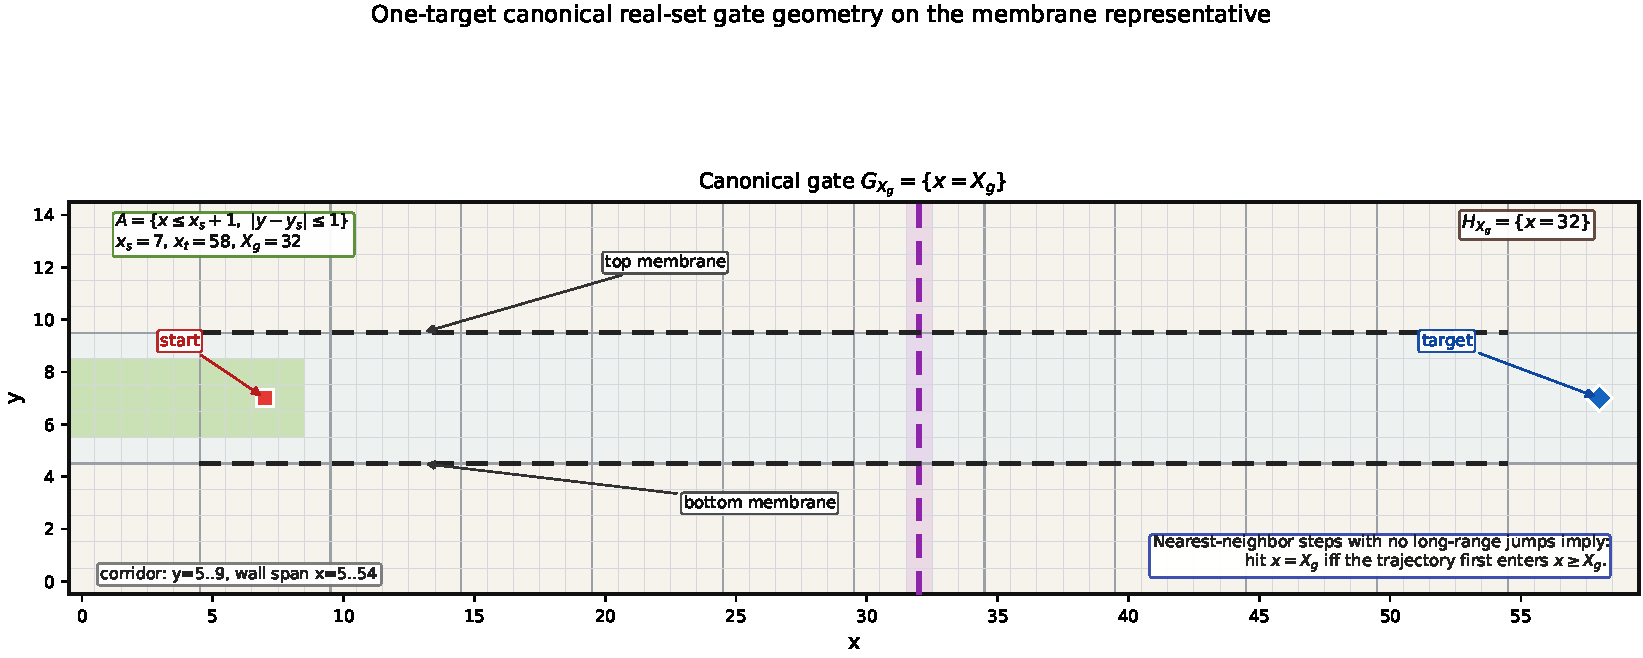
\includegraphics[width=0.90\linewidth]{../artifacts/figures/one_target_gate_geometry.pdf}
  \caption{Standard one-target geometry. The panel is drawn for the shared symmetric baseline and marks the lattice, corridor, start basin $A$, target, the true membrane interfaces, and the canonical x-gate $G_{X_g}=\{x=X_g\}$.}
\end{figure}

\paragraph{What the two asymmetry notions mean.}
The one-target branch now keeps the two physically different symmetry lines separate:
\begin{enumerate}
  \item \textbf{top/bottom symmetry}: whether the upper and lower membranes are the same;
  \item \textbf{same-membrane directional symmetry}: whether \texttt{corridor$\to$outside} and \texttt{outside$\to$corridor} have the same permeability on a given membrane.
\end{enumerate}
The first is scanned in the \texttt{tb} plane $(\kappa_{\rm top},\kappa_{\rm bottom})$, and the second in the \texttt{dir} plane $(\kappa_{c\to o},\kappa_{o\to c})$. They are numerically and physically different questions.

\section{Gate-free rollback classes and x-gate timing classes}
\paragraph{Why rollback is now gate-free.}
Rollback is now defined in a genuinely gate-free way: after a trajectory leaves the start basin $A$, does it later re-enter $A$? Under that definition the four rollback classes
\[
L0R0,\quad L0R1,\quad L1R0,\quad L1R1
\]
are mutually exclusive and exhaustive:
\begin{itemize}
  \item $L0R0$: no leak and no return to $A$;
  \item $L0R1$: no leak but a return to $A$ after leaving it;
  \item $L1R0$: membrane leak but no later return to $A$;
  \item $L1R1$: membrane leak and later return to $A$.
\end{itemize}

\paragraph{What the x-gate still does.}
The real-set x-gate is retained, but only for one purpose: to timestamp the \emph{first} leak relative to
\[
G_{X_g}=\{x=X_g\}.
\]
This yields the timing classes
\[
N=\text{NoLeak},\qquad
P=\text{first leak before gate},\qquad
Q=\text{first leak after gate}.
\]
Under the present nearest-neighbor lattice dynamics, hitting $x=X_g$ is equivalent to first entering $x\ge X_g$, so only the single canonical x-gate line remains in the main text.

\begin{figure}[!htbp]
  \centering
  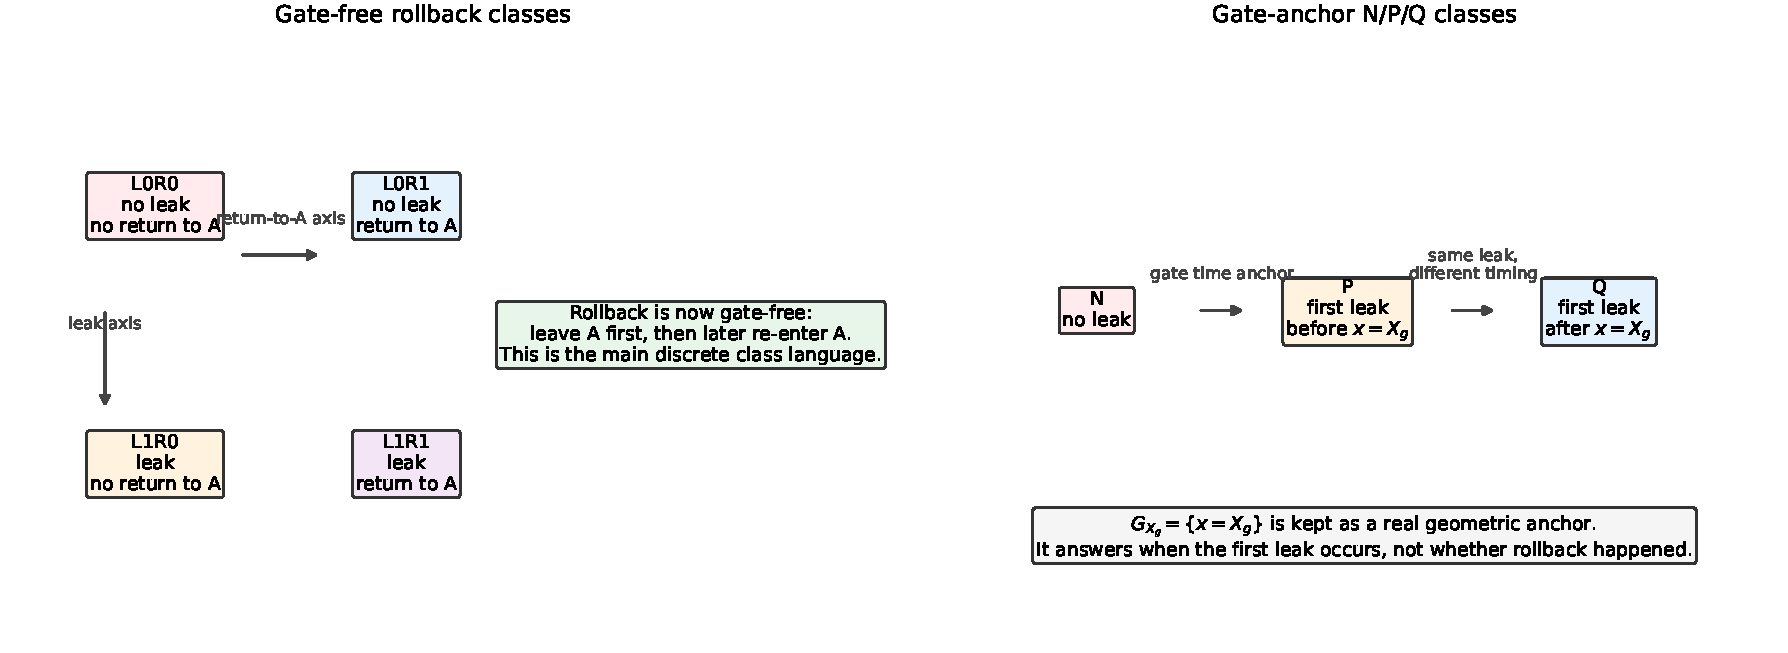
\includegraphics[width=0.88\linewidth]{../artifacts/figures/one_target_class_crosswalk.pdf}
  \caption{One-target class explainer. The rollback 4-class system answers ``did leak occur'' and ``did the path return to $A$''; the $N/P/Q$ system answers ``when did the first leak occur relative to the x-gate.'' The two are parallel diagnostics rather than competing definitions.}
\end{figure}

\section{Top/bottom parameter scan}
\paragraph{What this scan answers.}
This $15\times 15$ scan over
\[
\kappa_{\rm top},\kappa_{\rm bottom}\in
\{0,0.00025,\ldots,0.005\}
\]
asks how upper/lower membrane imbalance changes double-peak strength, phase-0 loss, and the balance between rollback and x-gate timing effects.

\begin{figure}[!htbp]
  \centering
  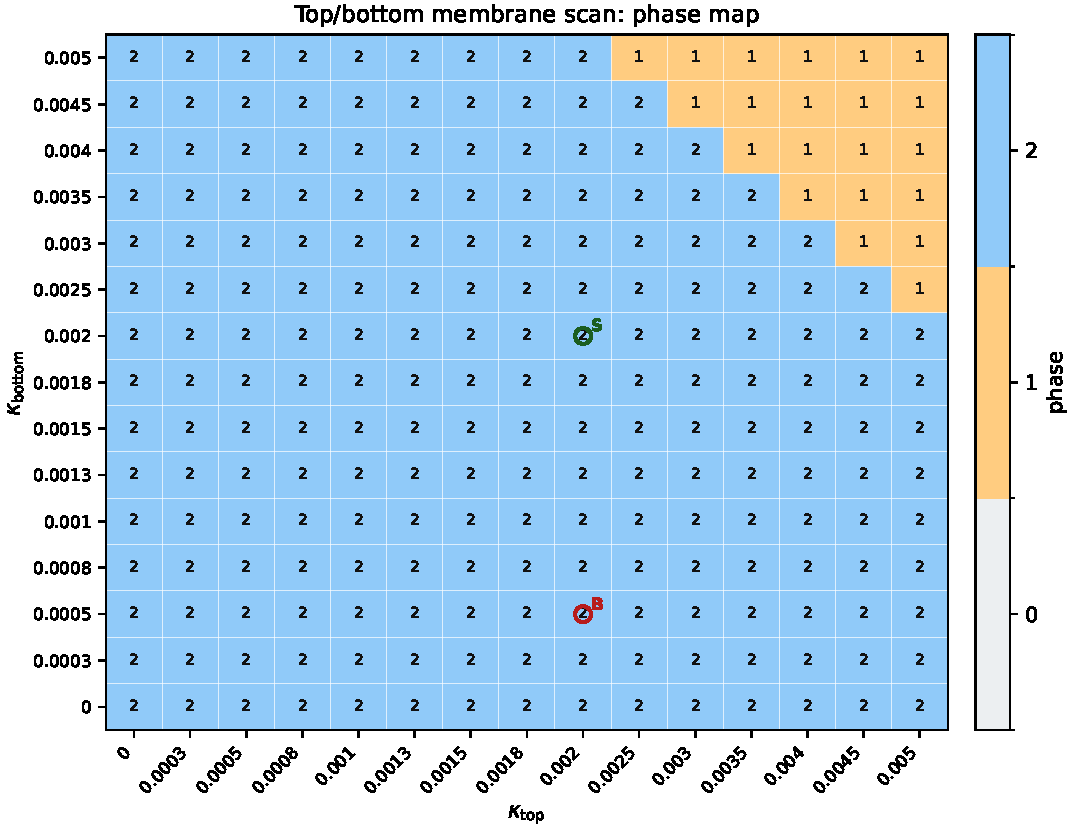
\includegraphics[width=0.88\linewidth]{../artifacts/figures/one_target_tb_phase_map.pdf}
  \caption{Top/bottom parameter-plane phase map. The shared symmetric baseline and the balanced top-open comparison point are explicitly marked.}
\end{figure}

\begin{figure}[!htbp]
  \centering
  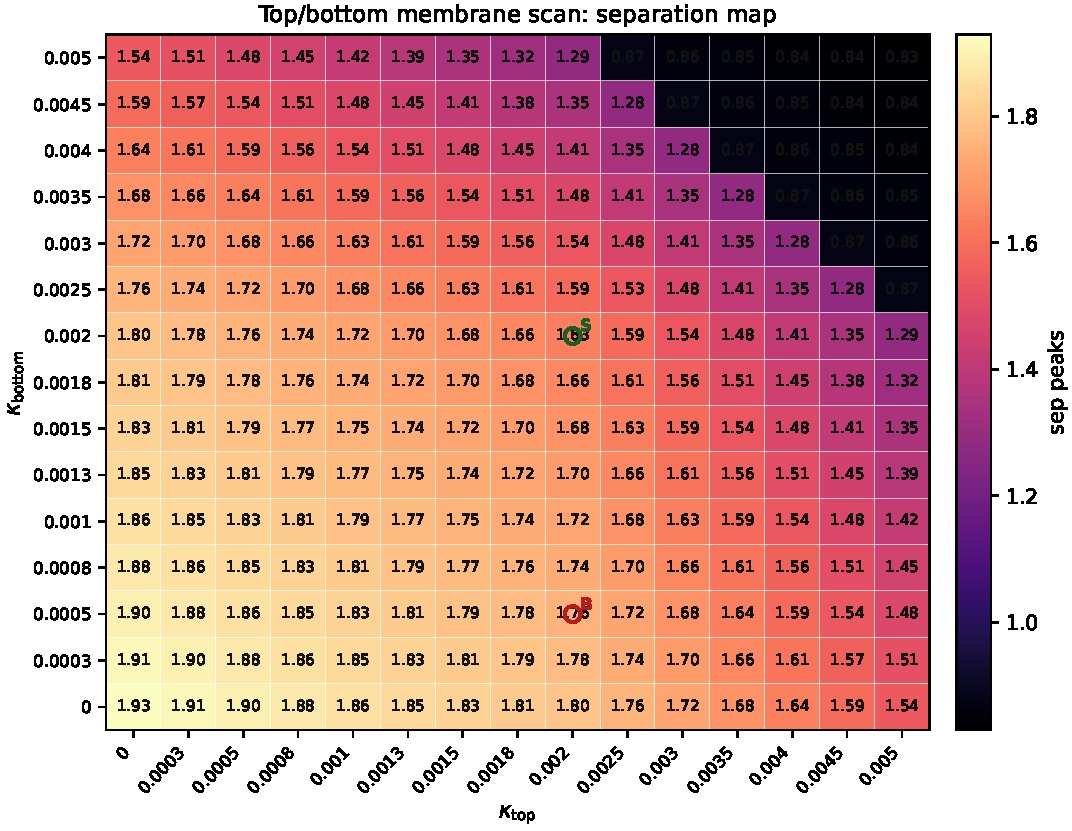
\includegraphics[width=0.88\linewidth]{../artifacts/figures/one_target_tb_sep_map.pdf}
  \caption{Peak-separation map on the same top/bottom plane. The color variation shows that moving away from the shared symmetric baseline first weakens and eventually can destroy the double-peak structure.}
\end{figure}

\section{Same-membrane directional scan}
\paragraph{Why this scan is kept separate.}
The top/bottom scan alone cannot answer whether the same membrane is easy to exit but hard to re-enter, or the reverse. That directional issue is therefore scanned explicitly in
\[
\kappa_{c\to o},\kappa_{o\to c}\in
\{0,0.00025,\ldots,0.005\}.
\]

\begin{figure}[!htbp]
  \centering
  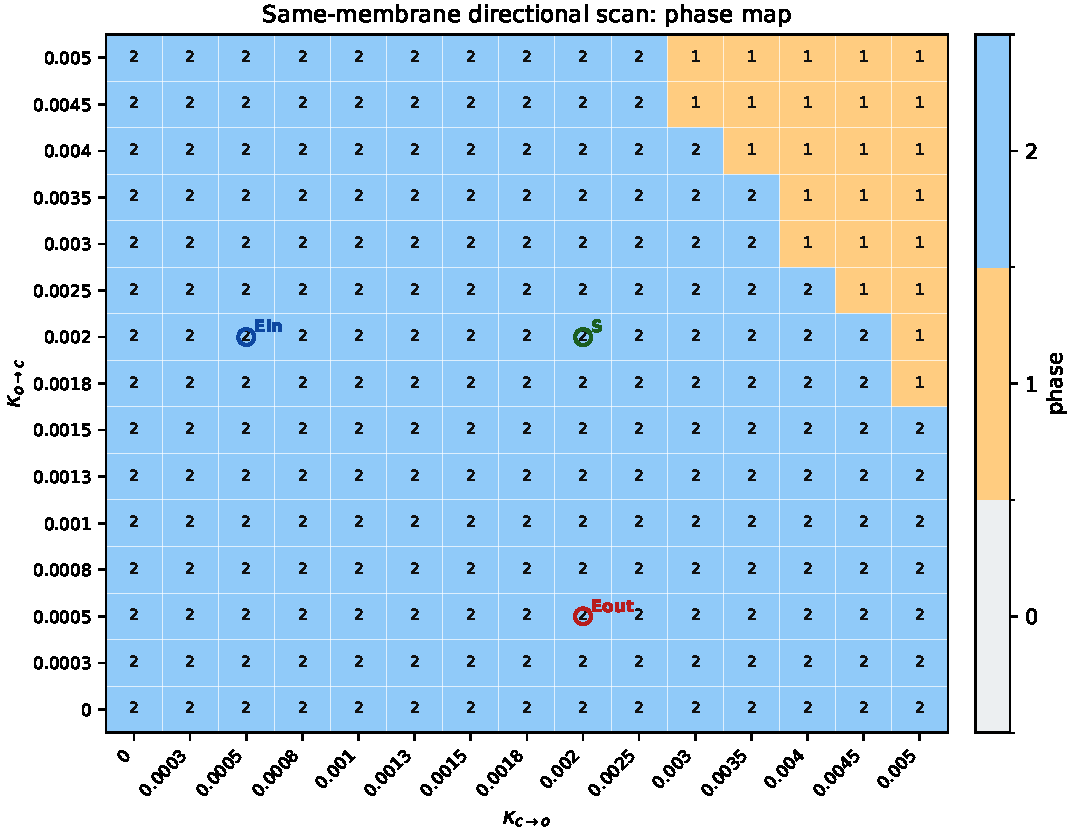
\includegraphics[width=0.88\linewidth]{../artifacts/figures/one_target_dir_phase_map.pdf}
  \caption{Phase map on the same-membrane directional plane. The shared symmetric baseline and the two directional comparison cases are marked explicitly.}
\end{figure}

\begin{figure}[!htbp]
  \centering
  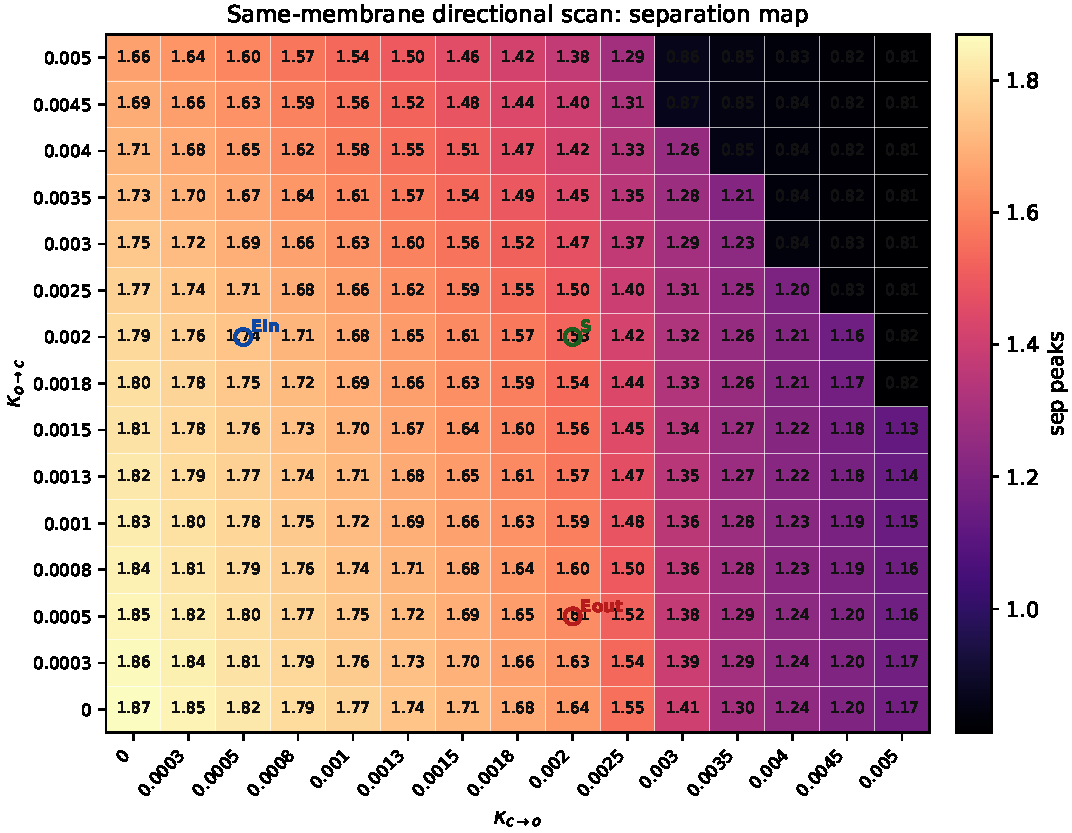
\includegraphics[width=0.88\linewidth]{../artifacts/figures/one_target_dir_sep_map.pdf}
  \caption{Peak-separation map on the directional plane. It shows directly how easy-out versus easy-in membranes alter the strength of the second peak.}
\end{figure}

\begin{table}[!htbp]
  \centering
  \caption{x-gate scan summary. For each canonical case the table reports dominant-$N$ counts and the ranges of $P/Q/$rollback across the full integer $X_g$ scan.}
  \begin{tabular}{llrrrr}
\toprule
case & scan range & dom. $N$ & $P$ range & $Q$ range & rollback range \\
\midrule
directional hard-out / easy-return & 9..57 & 49 & 0.1\%--2.8\% & 2.5\%--5.2\% & 28.2\%--76.4\% \\
directional easy-out / hard-return & 9..57 & 49 & 0.1\%--8.0\% & 1.3\%--9.1\% & 27.8\%--77.2\% \\
shared symmetric baseline & 9..57 & 49 & 0.2\%--8.6\% & 2.9\%--11.4\% & 27.5\%--77.0\% \\
top/bottom balanced asymmetry & 9..57 & 49 & 0.1\%--5.4\% & 1.8\%--7.2\% & 28.0\%--76.8\% \\
\bottomrule
\end{tabular}

\end{table}

\begin{figure}[!htbp]
  \centering
  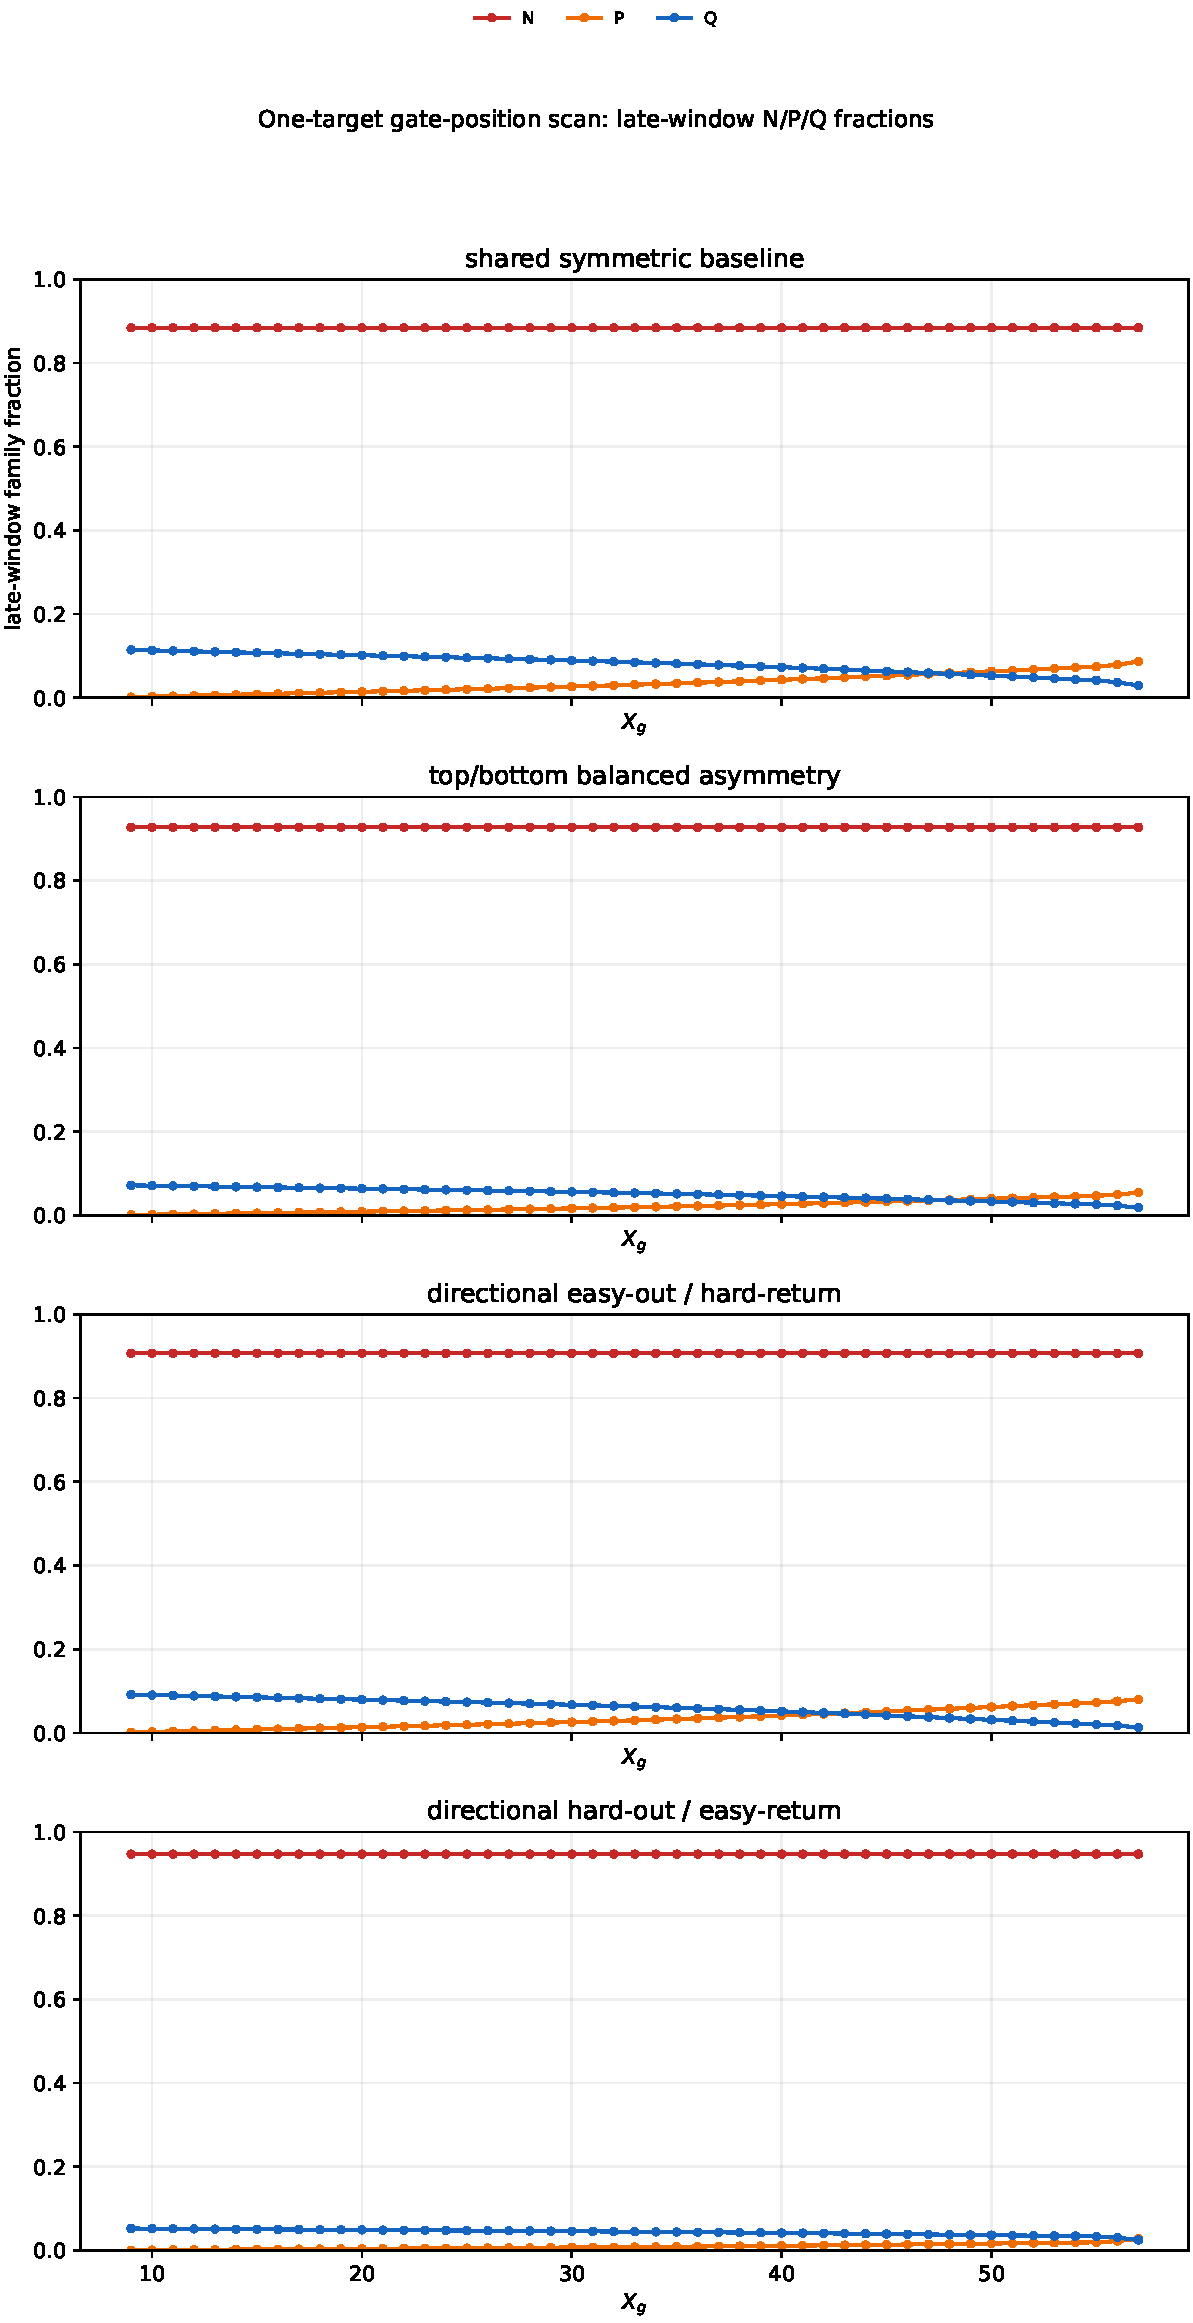
\includegraphics[width=0.92\linewidth]{../artifacts/figures/one_target_gate_scan_families.pdf}
  \caption{Full $X_g$ scan of the $N/P/Q$ decomposition. The rebuilt result is explicit about its negative message: the x-gate acts mainly as a geometric time anchor, not as a strong family-switching separator.}
\end{figure}

\begin{figure}[!htbp]
  \centering
  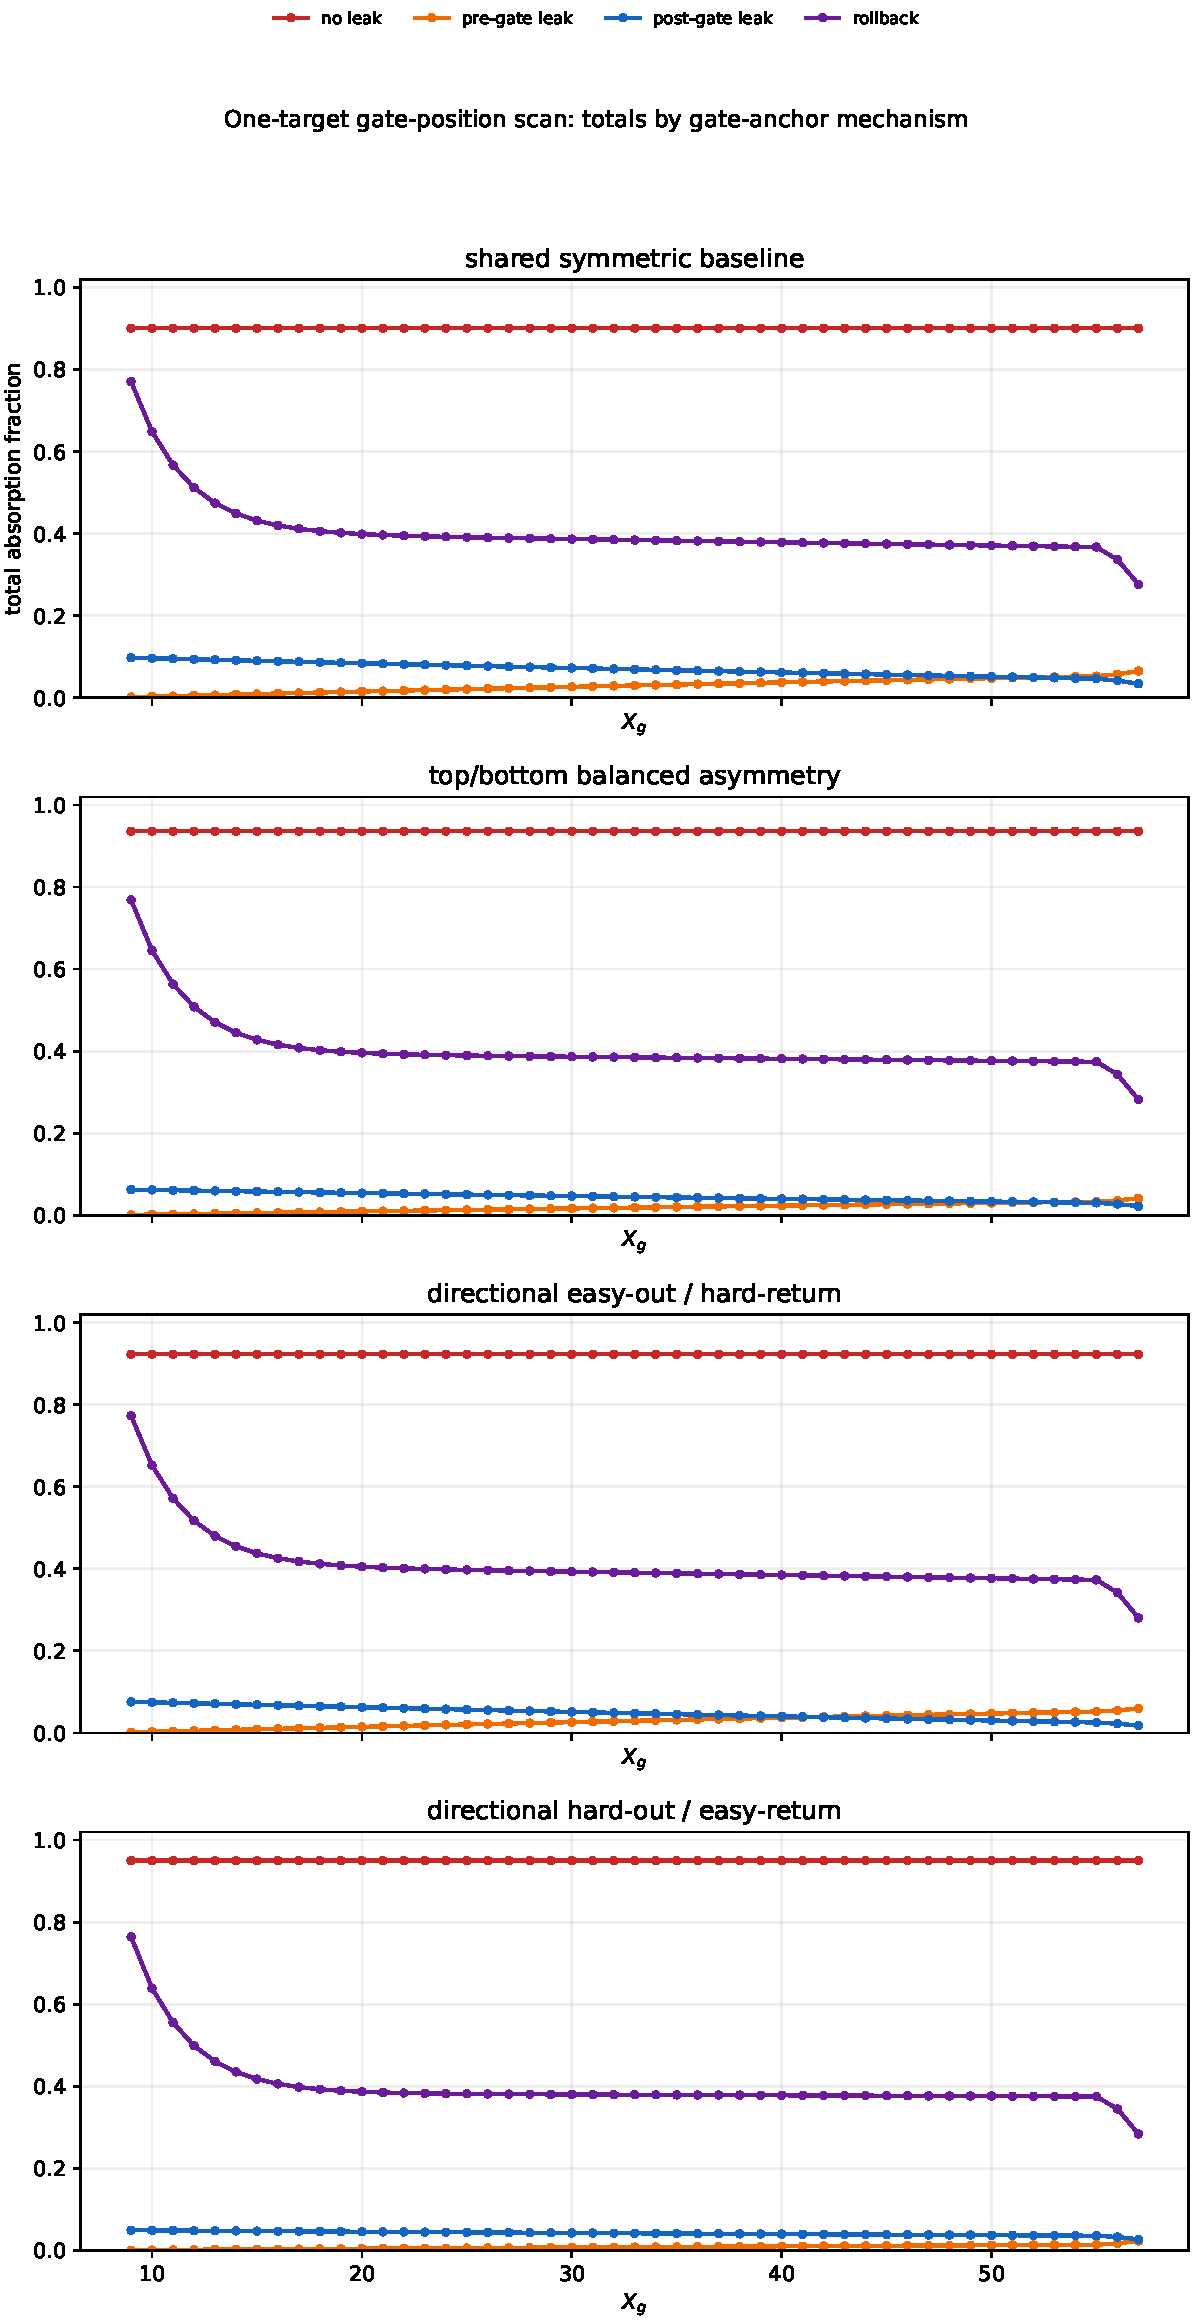
\includegraphics[width=0.92\linewidth]{../artifacts/figures/one_target_gate_scan_totals.pdf}
  \caption{Totals across the same $X_g$ scan. Varying the gate position mainly redistributes the $P/Q$ budget and changes rollback totals; it does not produce dramatic dominant-family flips.}
\end{figure}

\section{Start-position scan and phase-0 loss}
\paragraph{Only \texttt{phase=0} counts as true loss of bimodality.}
In this report \texttt{phase=2} means a clear double peak, \texttt{phase=1} means weakening but not disappearance, and only \texttt{phase=0} means that the second peak is genuinely lost. So the question ``when is the double peak lost'' is interpreted strictly as a phase-0 question.

\begin{figure}[!htbp]
  \centering
  
\includegraphics[width=0.95\linewidth]{../artifacts/figures/one_target_start_phase_map.pdf}
  \caption{Four-case start-position phase atlas. This figure answers where phase-0 loss begins and how it expands for different membrane configurations.}
\end{figure}

\paragraph{Why there is no full leak-balance atlas here.}
The start-position section is meant to answer one question cleanly: where phase-0 loss appears first. The rebuilt canonical pipeline therefore keeps the full start atlas phase-only exact, while leak timing and rollback budgets are discussed in the parameter scans and representative window decompositions rather than being recomputed on every start grid point.

\begin{table}[!htbp]
  \centering
  \caption{Phase-0 loss summary. For each canonical case the report records a centerline onset, an off-axis loss point, and a target-adjacent collapse point.}
  \begin{tabular}{lllll}
\toprule
case & phase-0 onset & off-axis loss & target-adjacent collapse & phase counts \\
\midrule
shared symmetric baseline & (46, 7) & (47, 5) & (57, 7) & 0:81/1:558/2:320 \\
top/bottom balanced asymmetry & (46, 7) & (46, 5) & (57, 7) & 0:83/1:555/2:321 \\
directional easy-out / hard-return & (46, 7) & (47, 5) & (57, 7) & 0:80/1:562/2:317 \\
directional hard-out / easy-return & (47, 7) & (47, 5) & (57, 7) & 0:77/1:555/2:327 \\
\bottomrule
\end{tabular}

\end{table}

\section{Representative refinements: rollback, x-gate, and directional flux}
\paragraph{Which mechanism is stronger.}
Under the present canonical rebuild, the stronger one-target discrete mechanism is the gate-free rollback system rather than the x-gate itself. The reason is simple: the rollback classes directly answer ``did leak happen'' and ``did the path return to $A$,'' while the x-gate mainly functions as a timing anchor for the first leak.

\begin{figure}[!htbp]
  \centering
  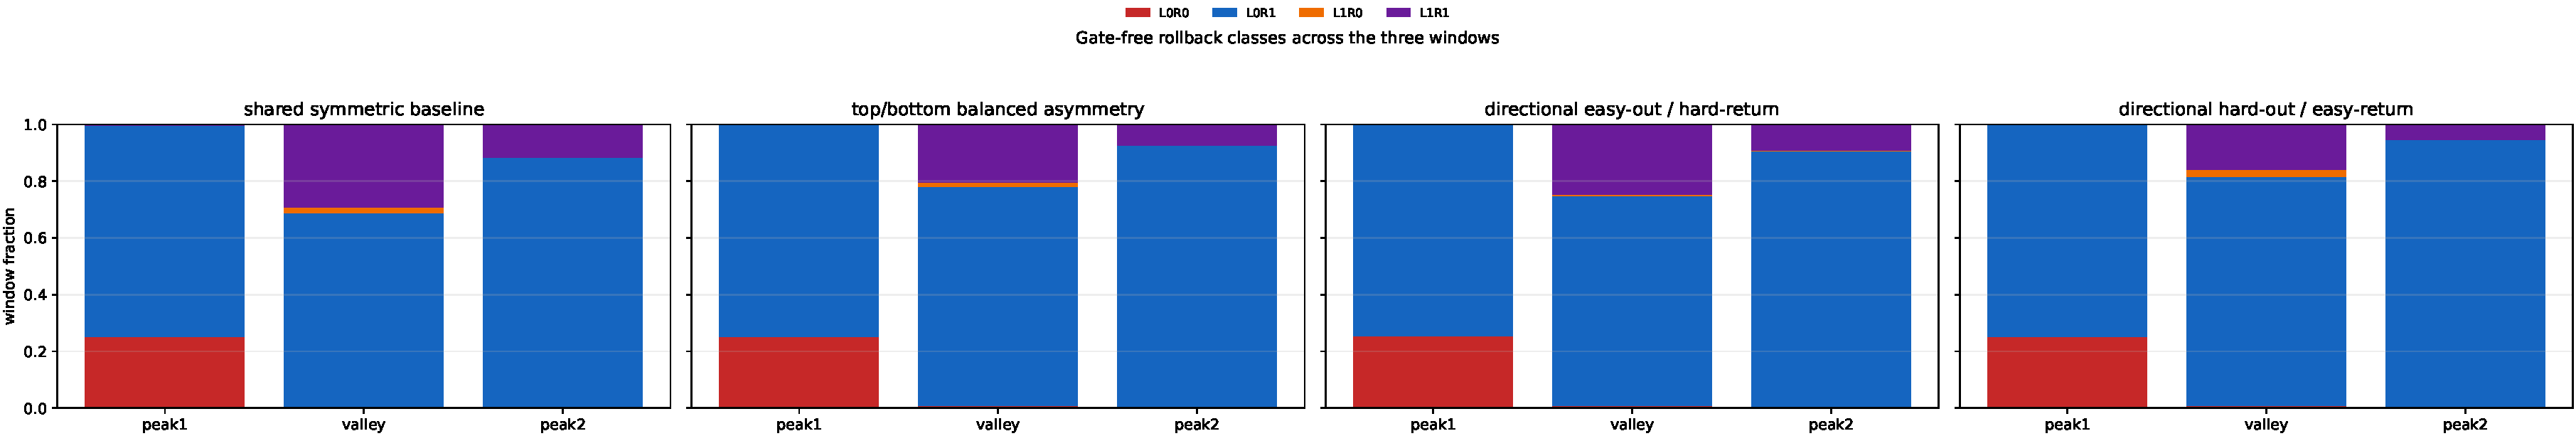
\includegraphics[width=0.92\linewidth]{../artifacts/figures/one_target_rollback_window_bars.pdf}
  \caption{Representative three-window rollback decomposition. The quantity $L0R1+L1R1$ is the direct measure of return-to-$A$ weight in the valley and late windows.}
\end{figure}

\begin{figure}[!htbp]
  \centering
  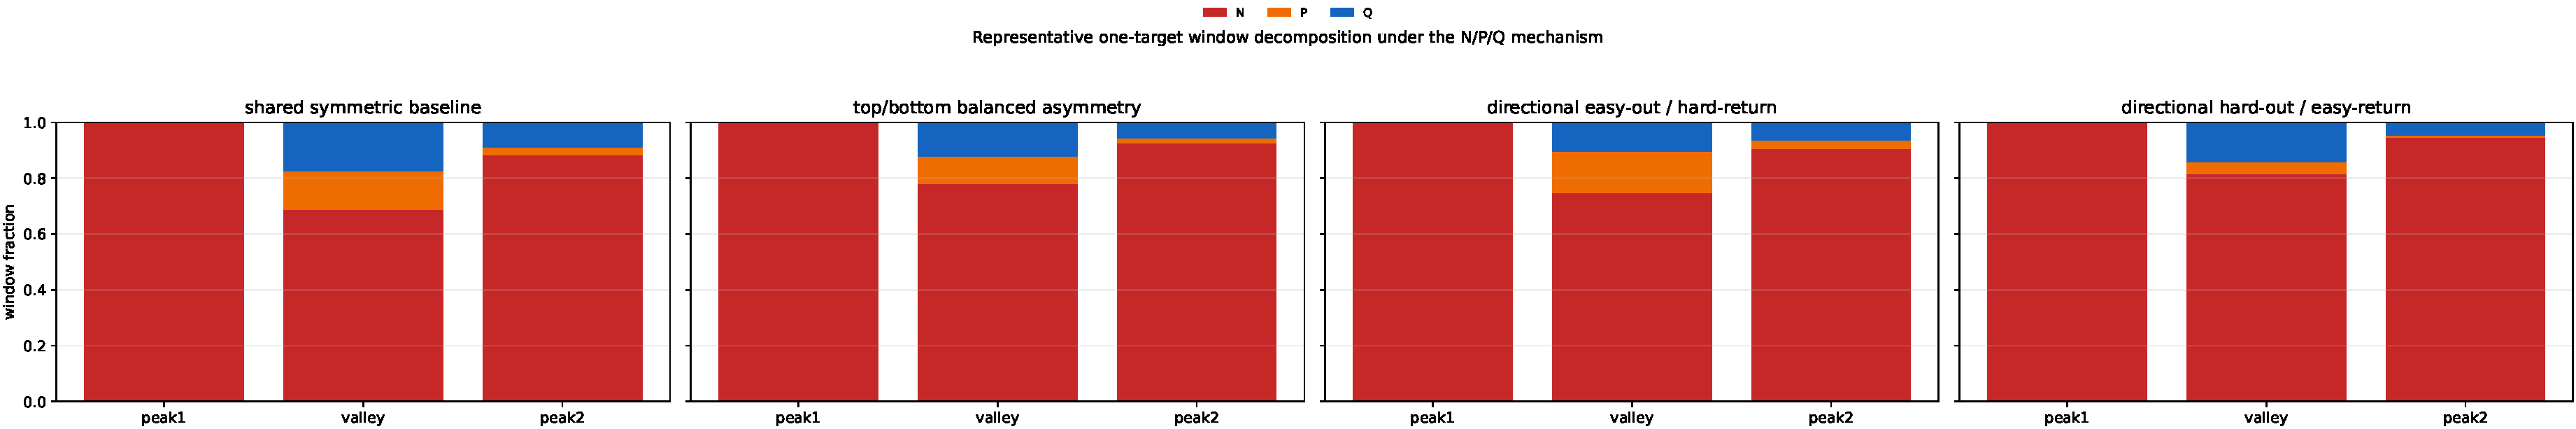
\includegraphics[width=0.92\linewidth]{../artifacts/figures/one_target_window_families.pdf}
  \caption{Representative three-window x-gate decomposition. Here $N/P/Q$ is used as a timing refinement, not as the primary discrete mechanism language.}
\end{figure}

\begin{figure}[!htbp]
  \centering
  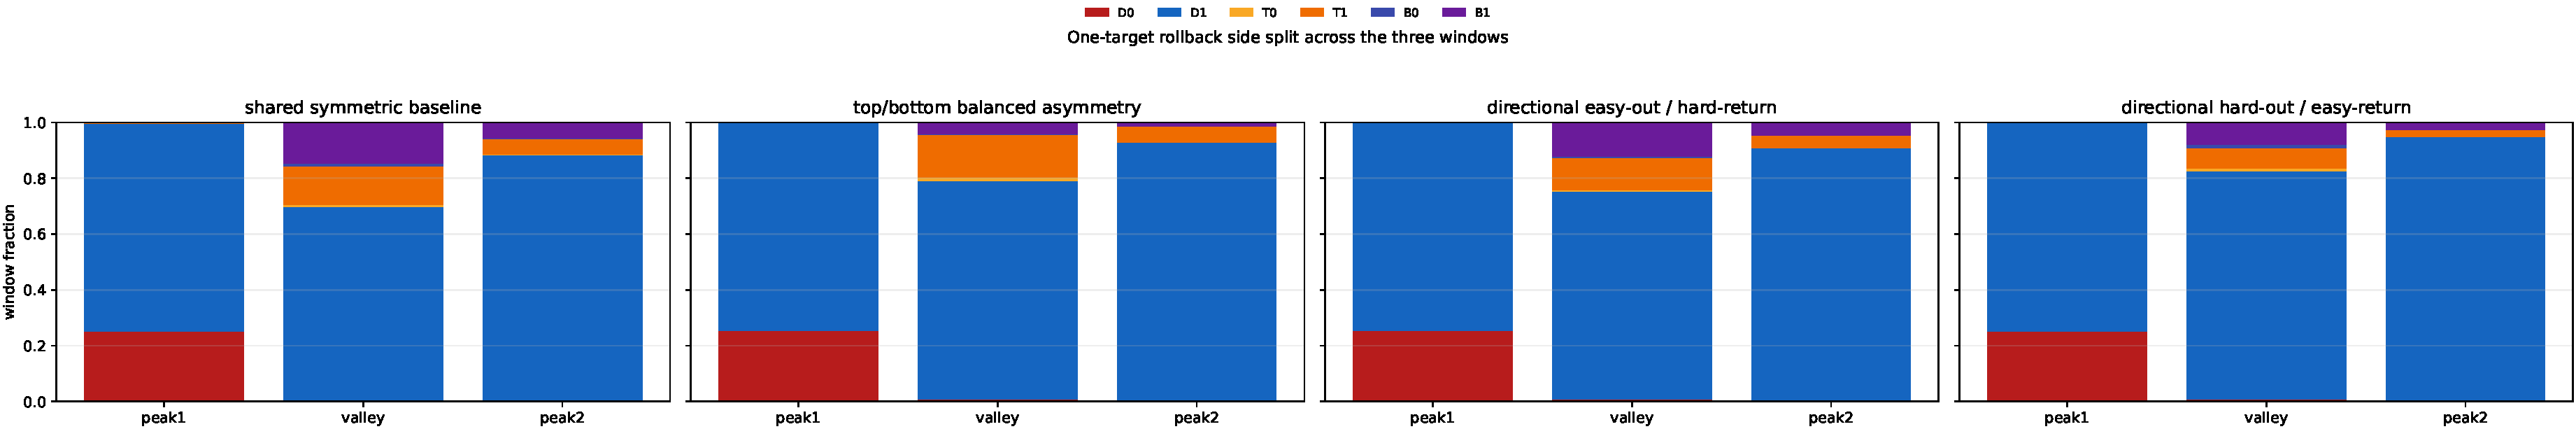
\includegraphics[width=0.92\linewidth]{../artifacts/figures/one_target_side_window_bars.pdf}
  \caption{Side-aware rollback refinement. For the shared symmetric baseline, top/bottom is mainly a symmetry check; for the top/bottom asymmetric comparison case, it becomes a real side preference.}
\end{figure}

\begin{figure}[!htbp]
  \centering
  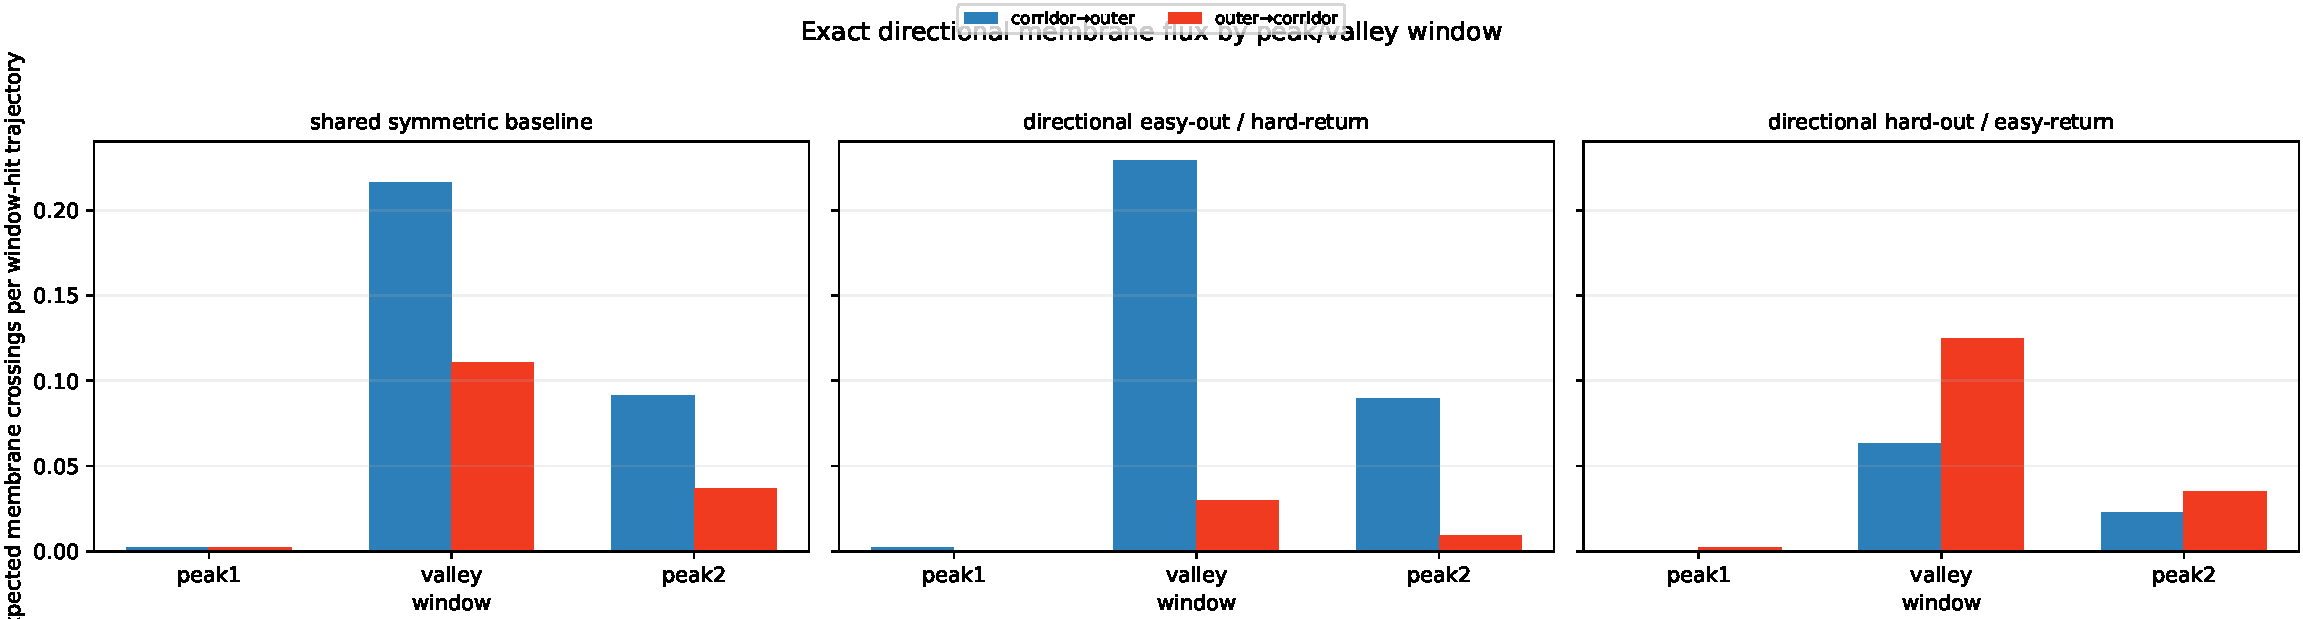
\includegraphics[width=0.92\linewidth]{../artifacts/figures/one_target_directional_window_flux.pdf}
  \caption{Directional window-flux diagnostics. This figure explains why easy-out versus easy-in membranes alter the second peak, rather than leaving the effect hidden at the parameter-name level.}
\end{figure}

\begin{figure}[!htbp]
  \centering
  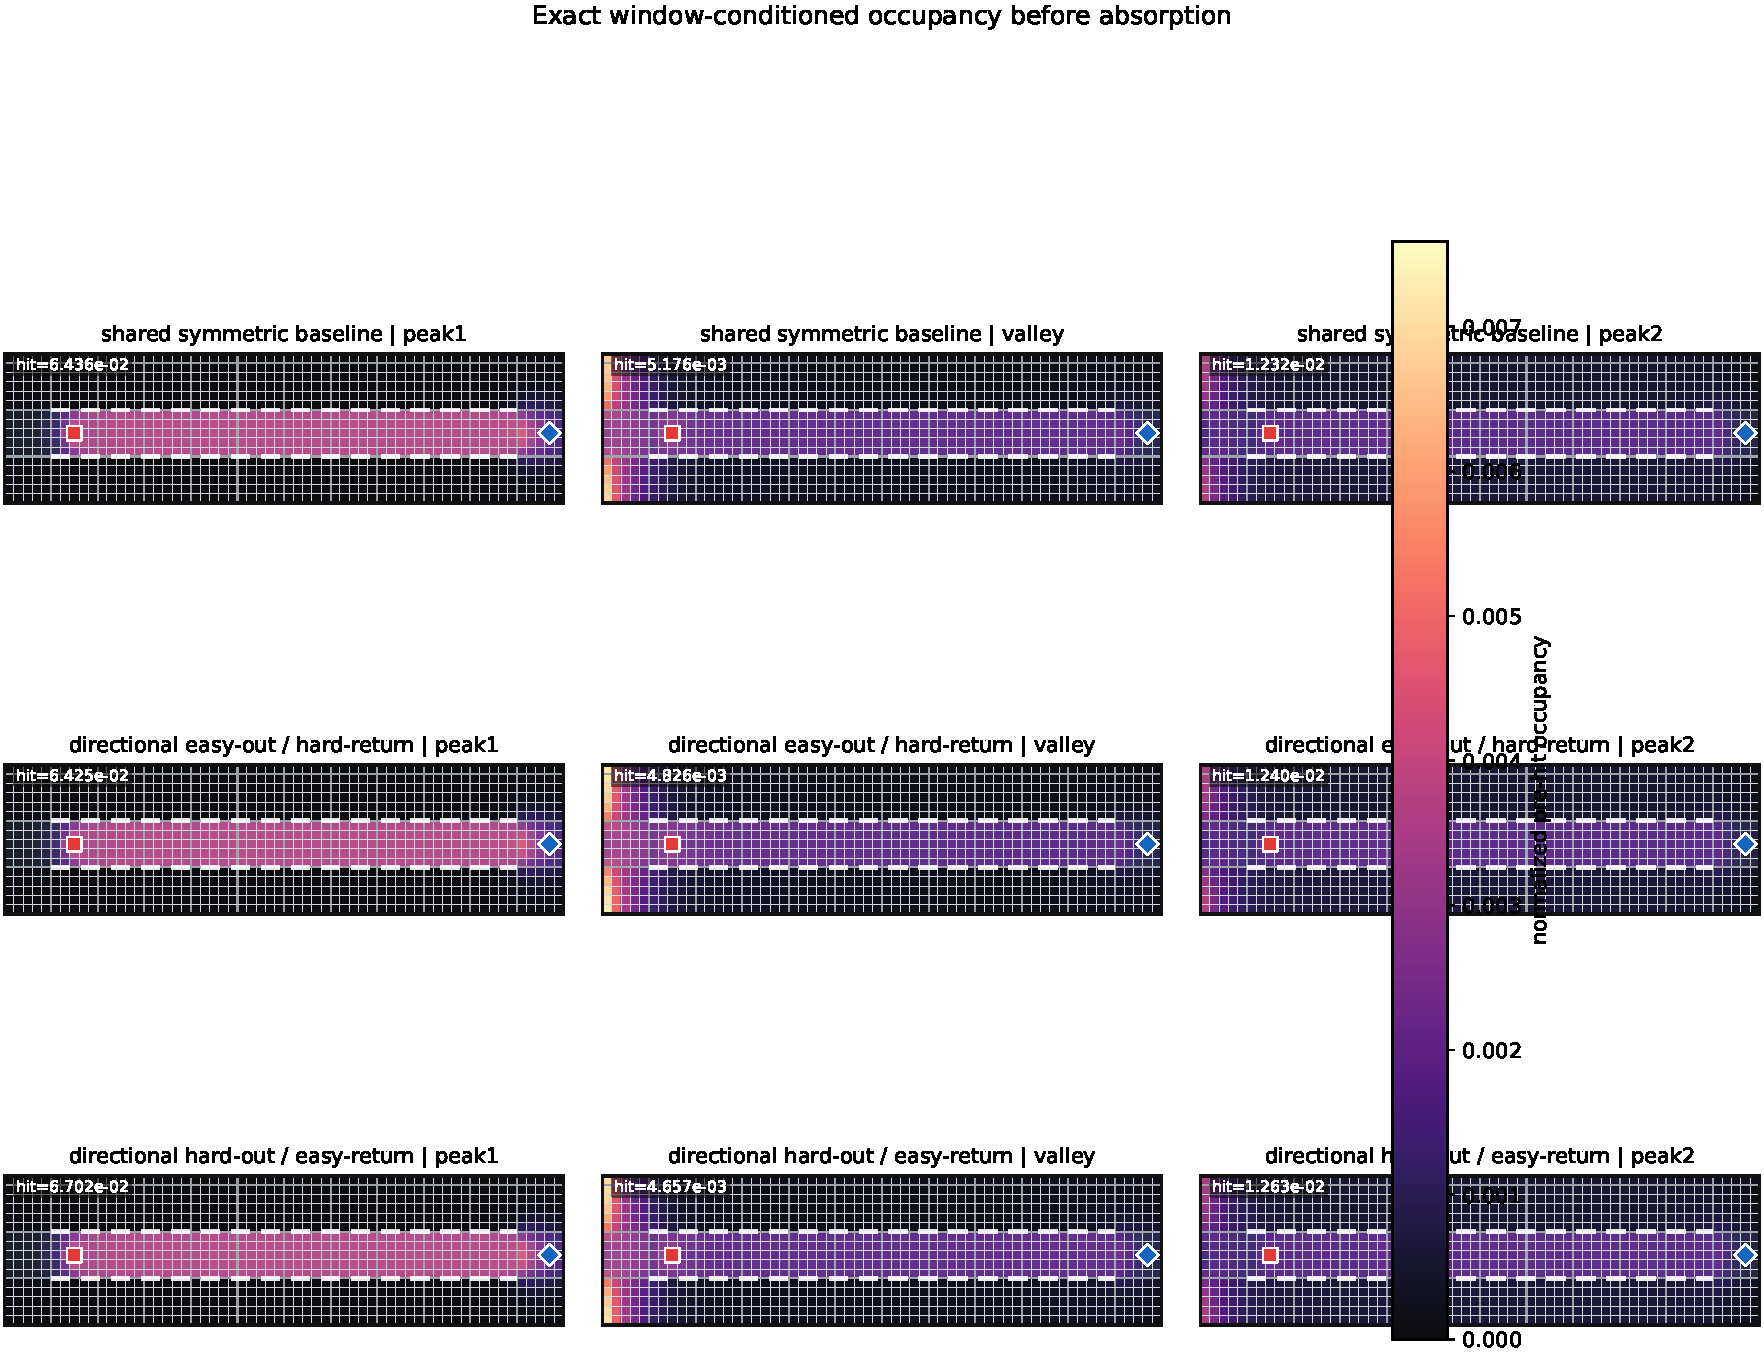
\includegraphics[width=0.95\linewidth]{../artifacts/figures/one_target_directional_window_occupancy_atlas.pdf}
  \caption{Representative window-occupancy atlas for the directional line. It puts the slow branch back onto the actual lattice geometry.}
\end{figure}

\begin{table}[!htbp]
  \centering
  \caption{Representative one-target recheck. The table reports phase, separation, peak2 rollback share, and the ranges of $P/Q/$rollback across the full $X_g$ scan.}
  \begin{tabular}{lrrrrrr}
\toprule
case & phase & sep & peak2 rollback share & $P$ range & $Q$ range & rollback range \\
\midrule
shared symmetric baseline & 2 & 1.633 & 99.7\% & 0.2\%--8.7\% & 3.1\%--11.6\% & 27.7\%--77.1\% \\
top/bottom balanced asymmetry & 2 & 1.756 & 99.8\% & 0.1\%--5.4\% & 2.0\%--7.3\% & 28.2\%--76.9\% \\
directional easy-out / hard-return & 2 & 1.710 & 99.9\% & 0.1\%--8.0\% & 1.4\%--9.2\% & 28.0\%--77.3\% \\
directional hard-out / easy-return & 2 & 1.800 & 99.7\% & 0.1\%--2.8\% & 2.7\%--5.4\% & 28.4\%--76.4\% \\
\bottomrule
\end{tabular}

\end{table}

\section{Two-target: the gate-lifted family line stays unchanged}
The two-target branch is numerically unchanged by this one-target rewrite. Its canonical conclusion remains that the late coarse family is stably \texttt{F\_no\_return}, not \texttt{F\_rollback}. This section therefore keeps the canonical figures, scan slices, and verification tables without changing the underlying mechanism language.

\begin{table}[!htbp]
  \centering
  \caption{Two-target representative cases.}
  \begin{tabular}{lrrrrrrr}
\toprule
case & phase & $P_{near}$ & $P_{far}$ & $t_{p1}$ & $t_v$ & $t_{p2}$ & sep$_{gate}$ \\
\midrule
anchor & 2 & 0.324 & 0.676 & 7 & 196 & 469 & 2.493 \\
clear\_instance & 2 & 0.350 & 0.650 & 13 & 207 & 471 & 2.380 \\
near\_mass\_loss & 2 & 0.089 & 0.911 & 27 & 193 & 470 & 2.229 \\
\bottomrule
\end{tabular}

\end{table}

\begin{table}[!htbp]
  \centering
  \caption{Two-target validation.}
  \begin{tabular}{lrrrrr}
\toprule
case & $q_{far}(start)$ & $P_{far}$ & gap & closure & MC err \\
\midrule
anchor & 0.676009 & 0.676009 & 0.000000 & 0.000000 & 0.006816 \\
clear\_instance & 0.650264 & 0.650264 & 0.000000 & 0.000000 & 0.004222 \\
near\_mass\_loss & 0.911262 & 0.911262 & 0.000000 & 0.000000 & 0.005743 \\
\bottomrule
\end{tabular}

\end{table}

\begin{table}[!htbp]
  \centering
  \caption{Phase counts on the 63-point $(d,\Delta y)$ atlas.}
  \begin{tabular}{rr}
\toprule
phase & count \\
\midrule
0 & 2 \\
2 & 61 \\
\bottomrule
\end{tabular}

\end{table}

\begin{figure}[!htbp]
  \centering
  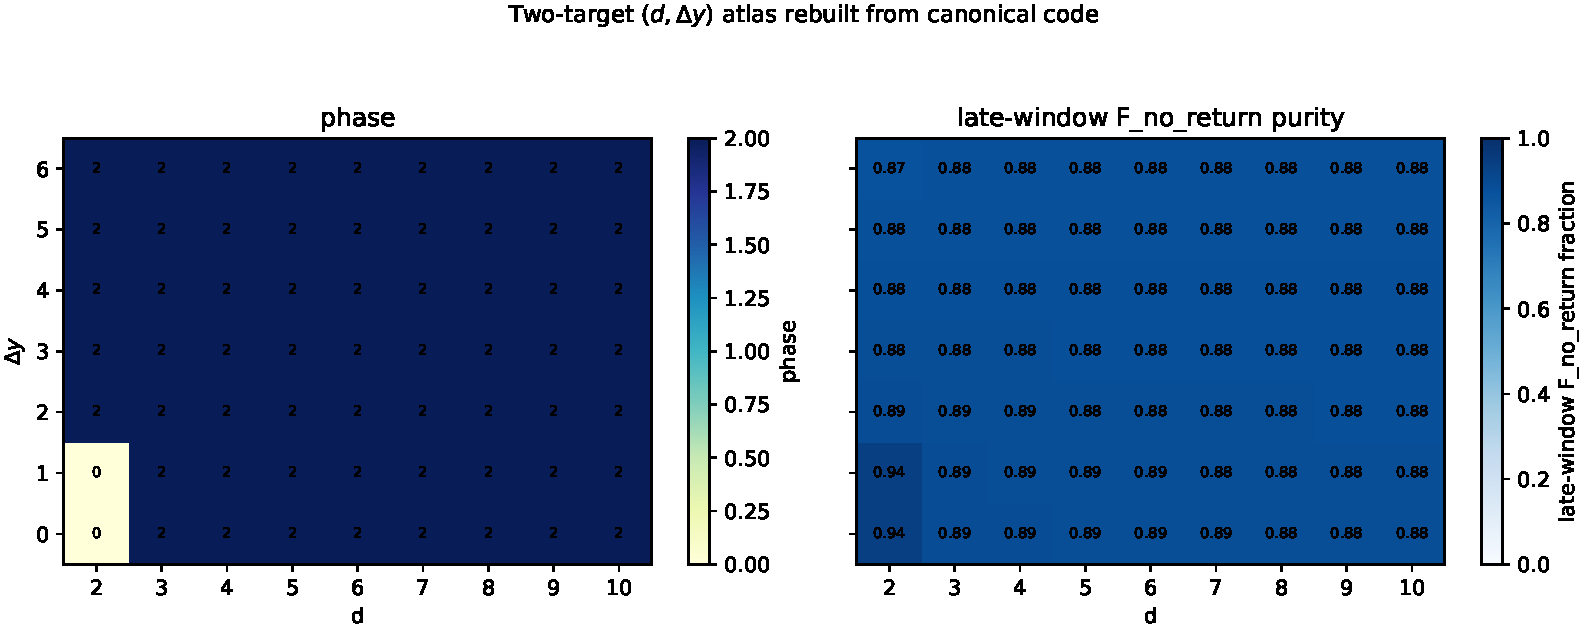
\includegraphics[width=0.88\linewidth]{../artifacts/figures/two_target_dx_dy_phase_purity.pdf}
  \caption{The 63-point two-target atlas. The current canonical rebuild still keeps phase-0 loss confined to a small subset of the grid.}
\end{figure}

\begin{figure}[!htbp]
  \centering
  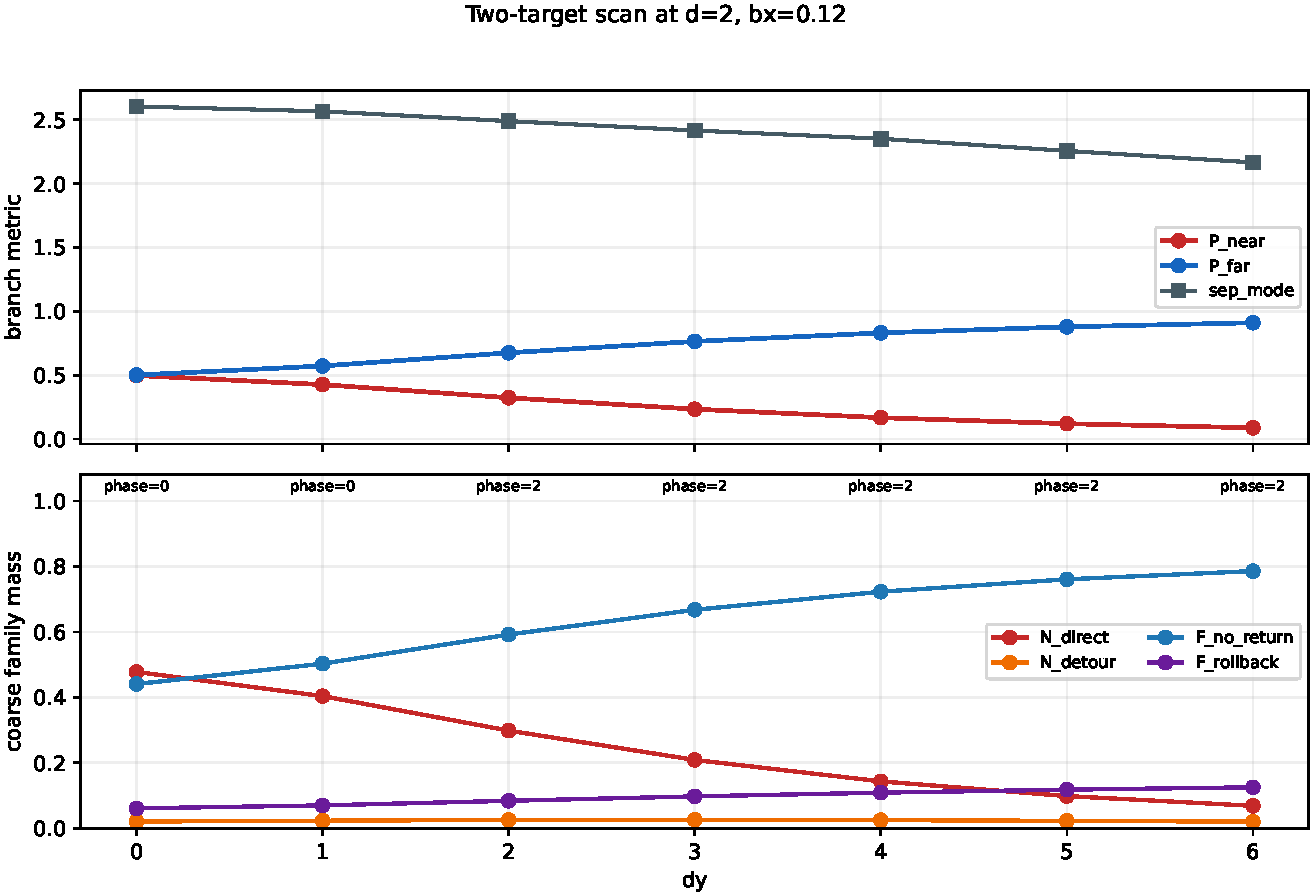
\includegraphics[width=0.88\linewidth]{../artifacts/figures/two_target_scan_dy_d2_bx0p12.pdf}
  \caption{The $\Delta y$ scan at fixed $d=2$.}
\end{figure}

\begin{figure}[!htbp]
  \centering
  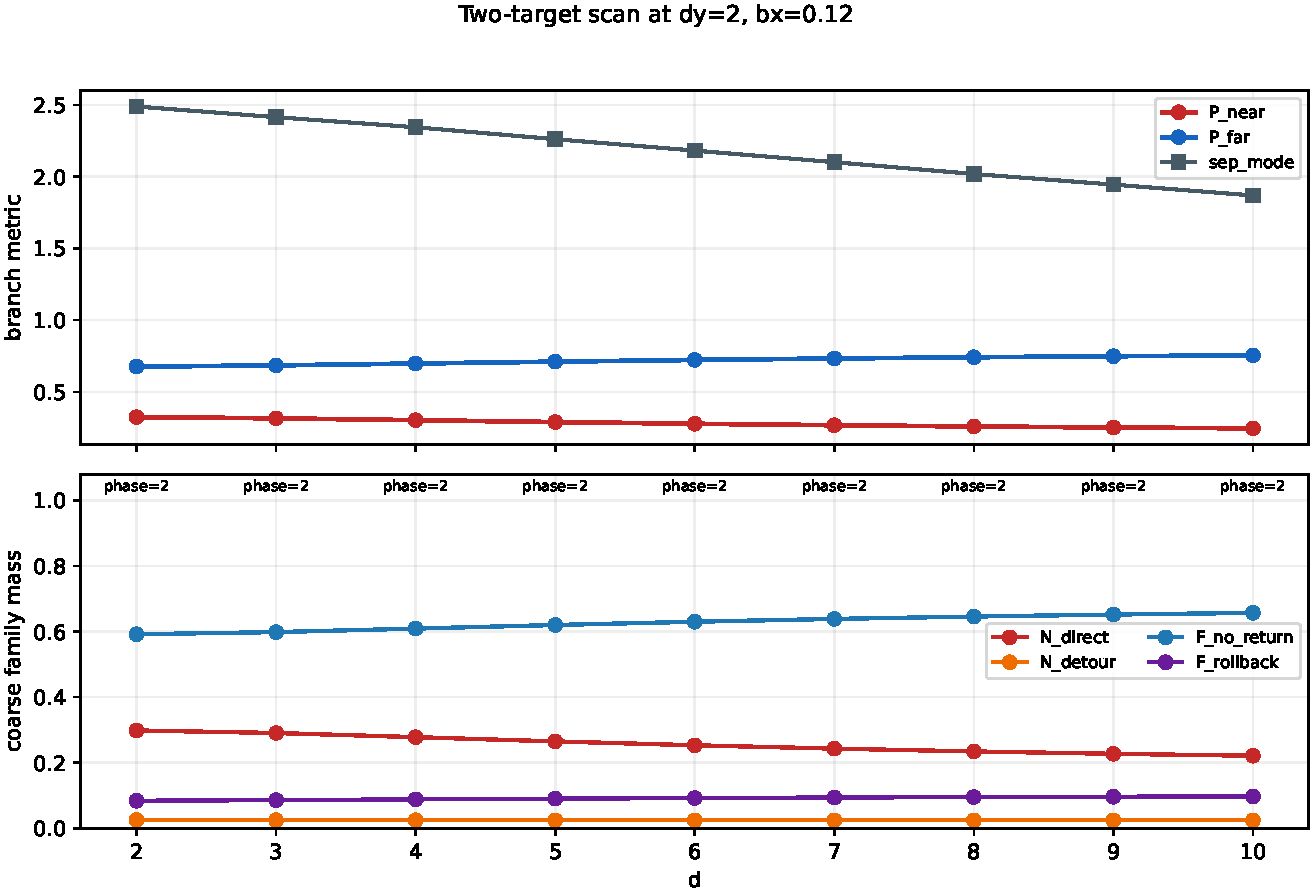
\includegraphics[width=0.88\linewidth]{../artifacts/figures/two_target_scan_d_dy2_bx0p12.pdf}
  \caption{The $d$ scan at fixed $\Delta y=2$.}
\end{figure}

\begin{figure}[!htbp]
  \centering
  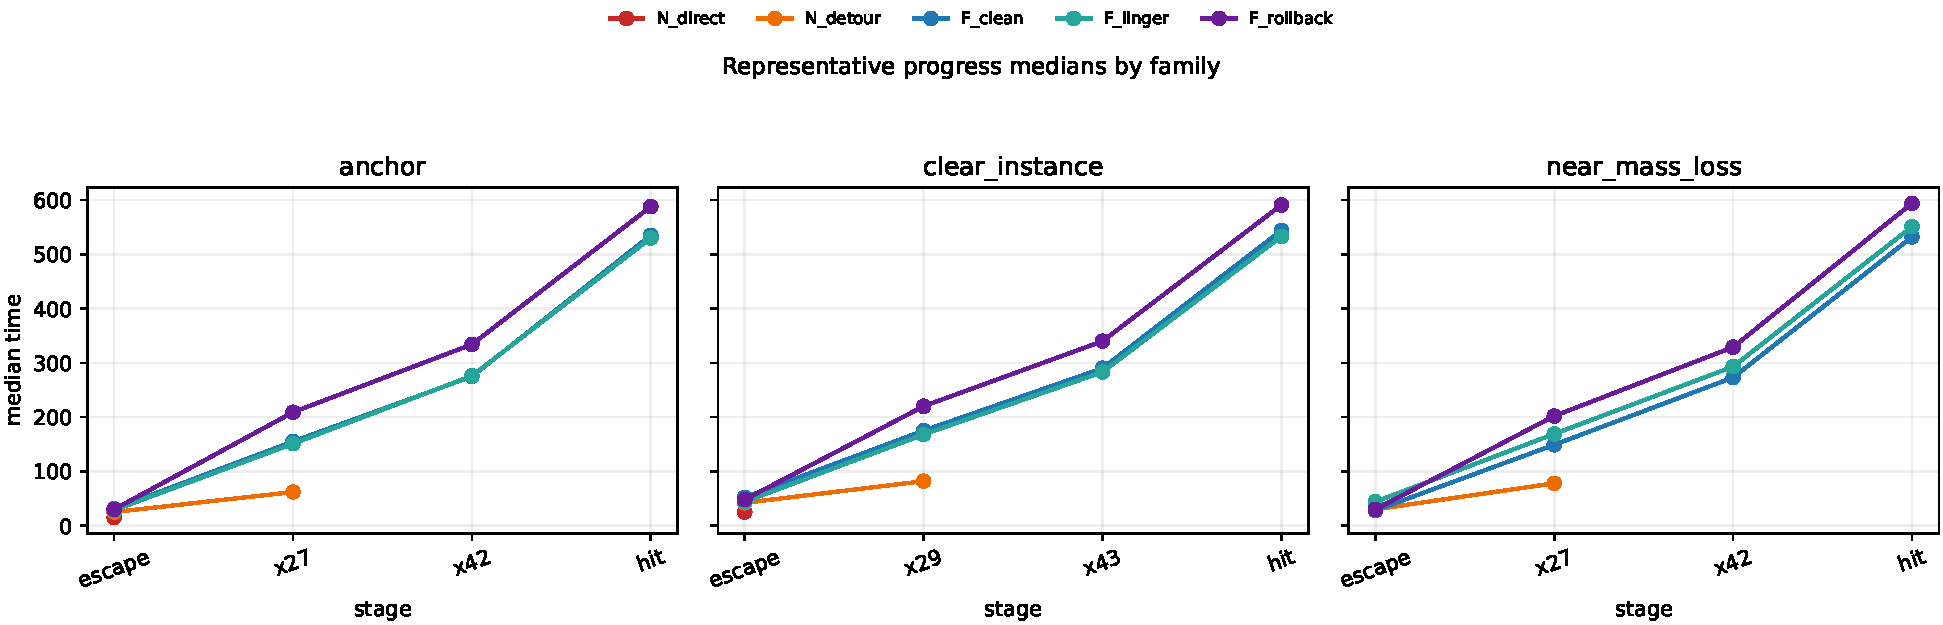
\includegraphics[width=0.86\linewidth]{../artifacts/figures/two_target_progress_medians.pdf}
  \caption{Representative progress medians.}
\end{figure}

\begin{figure}[!htbp]
  \centering
  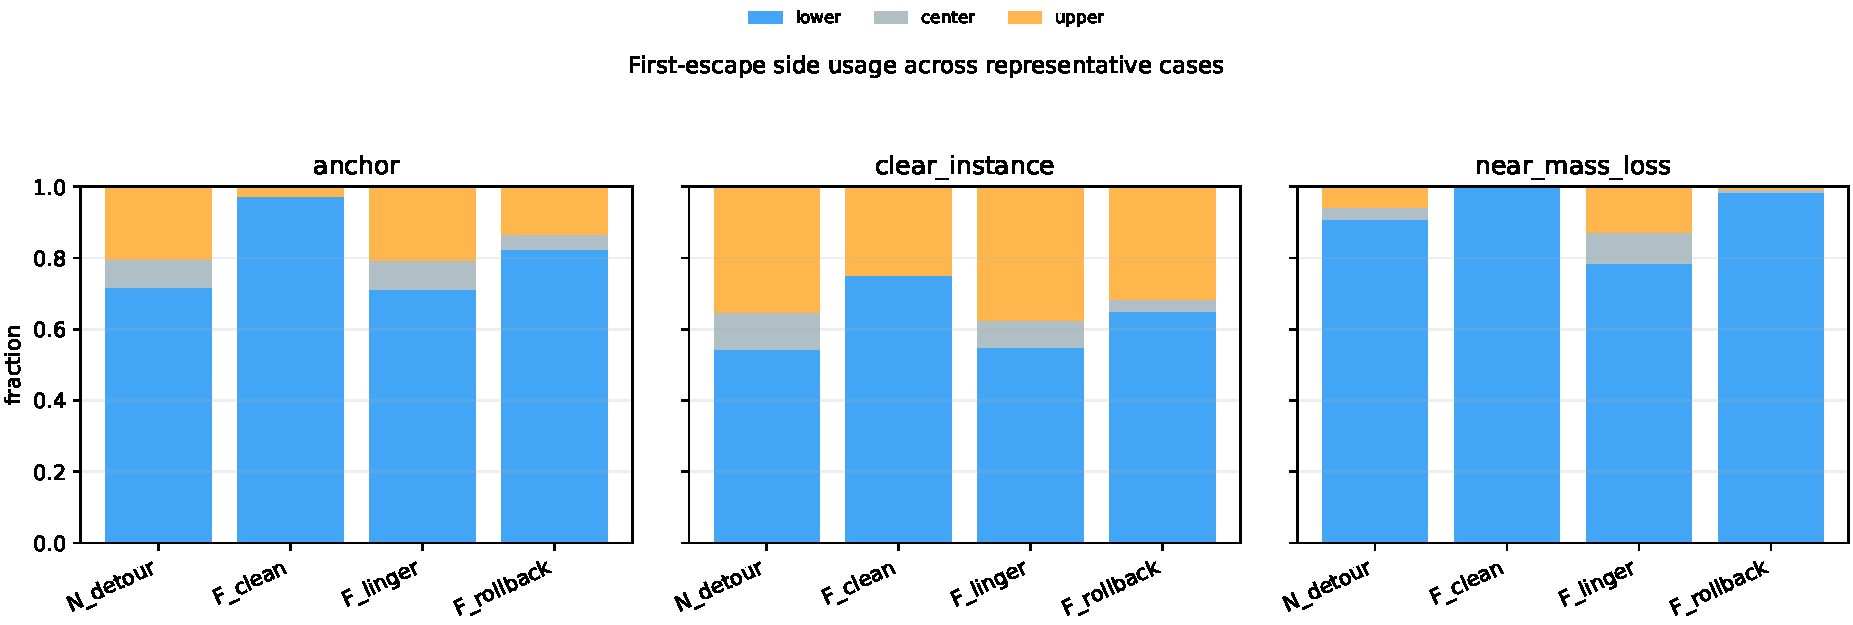
\includegraphics[width=0.86\linewidth]{../artifacts/figures/two_target_first_escape_side_usage.pdf}
  \caption{Representative first-escape side usage.}
\end{figure}

\begin{figure}[!htbp]
  \centering
  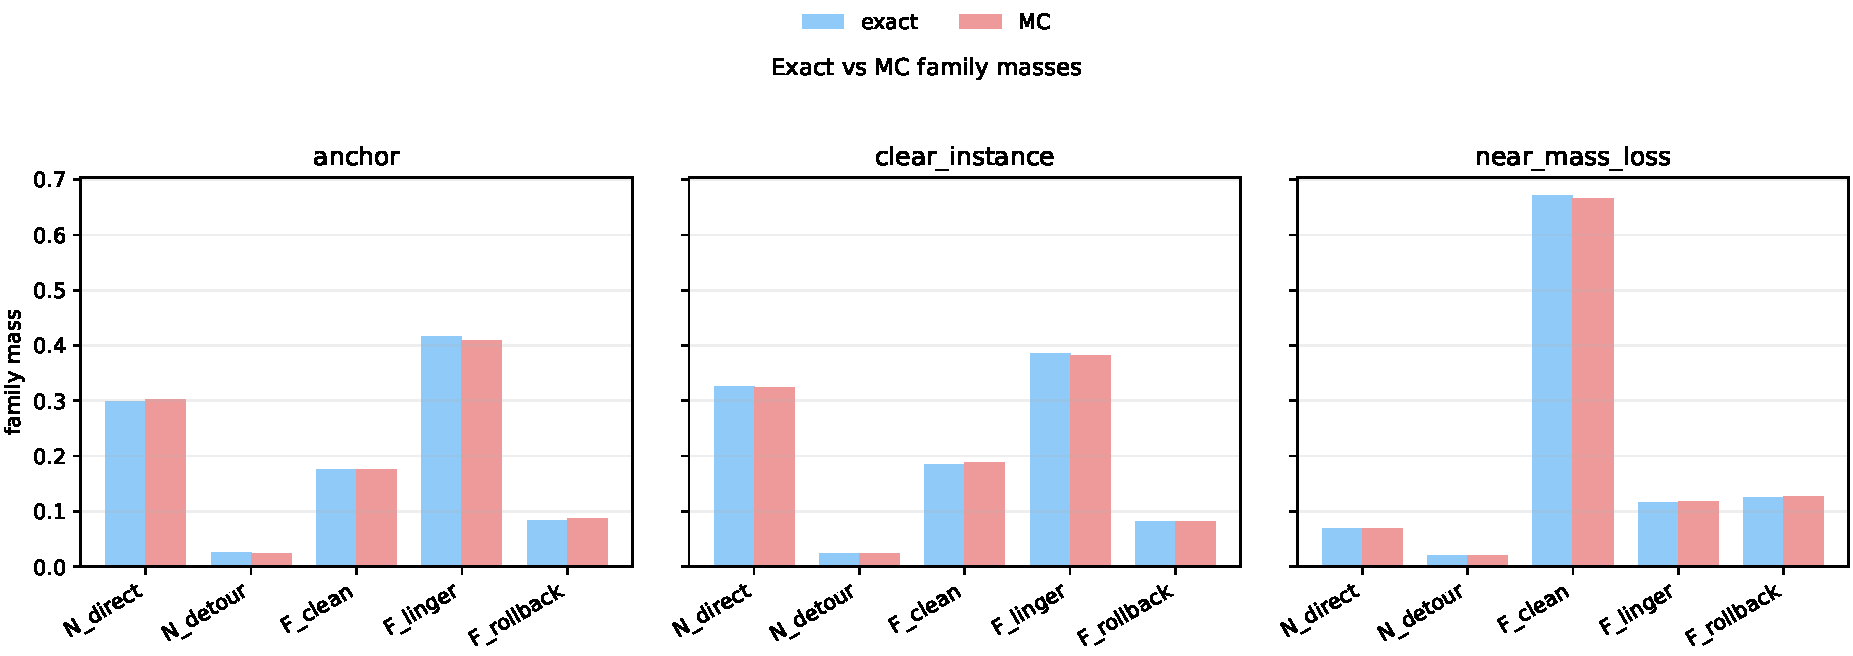
\includegraphics[width=0.86\linewidth]{../artifacts/figures/two_target_mc_vs_exact.pdf}
  \caption{MC-vs-exact comparison.}
\end{figure}

\begin{figure}[!htbp]
  \centering
  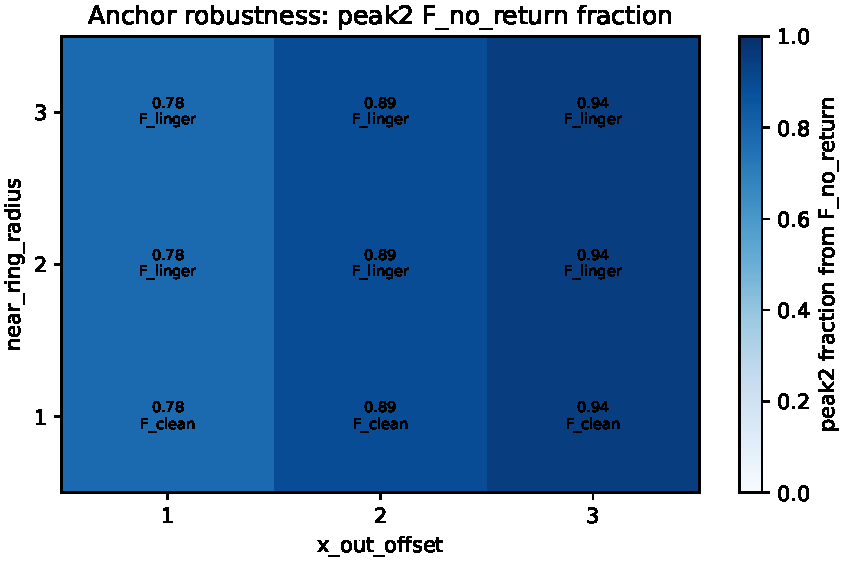
\includegraphics[width=0.86\linewidth]{../artifacts/figures/two_target_anchor_gate_robustness.pdf}
  \caption{Gate robustness for the anchor case.}
\end{figure}

\begin{table}[!htbp]
  \centering
  \caption{Representative two-target recheck.}
  \begin{tabular}{lrrrrr}
\toprule
case & source $P_{far}$ & recheck $P_{far}$ & $q_{far}(start)$ gap & late family & MC err \\
\midrule
anchor & 0.676009 & 0.676009 & 0.000000 & F\_no\_return & 0.0068 \\
clear\_instance & 0.650264 & 0.650264 & 0.000000 & F\_no\_return & 0.0042 \\
near\_mass\_loss & 0.911262 & 0.911262 & 0.000000 & F\_no\_return & 0.0057 \\
\bottomrule
\end{tabular}

\end{table}

\section{Repository integration and appendix note}
\paragraph{Repository integration.}
The six original downloaded files remain archived under
\texttt{notes/source\_imports/2026-03-16/raw/}.
The new \texttt{artifacts/} and \texttt{manuscript/} trees are rebuilt directly from
\texttt{vkcore.grid2d.one\_two\_target\_gating.*}.

\paragraph{The final one-target language of this version.}
The one-target final language can now be summarized in one sentence:
\begin{quote}
the standard configuration is the shared symmetric baseline; rollback is the main discrete mechanism; the x-gate is a timing anchor; bimodality loss means \texttt{phase=0}; and extreme $\kappa=0$ points are controls rather than main representatives.
\end{quote}

\section{Appendix: committor control}
The committor construction remains in the repository, but only as an appendix-level control. It is still useful for historical continuity and numerical sanity checks, yet it no longer defines the main one-target gate language.

\begin{figure}[!htbp]
  \centering
  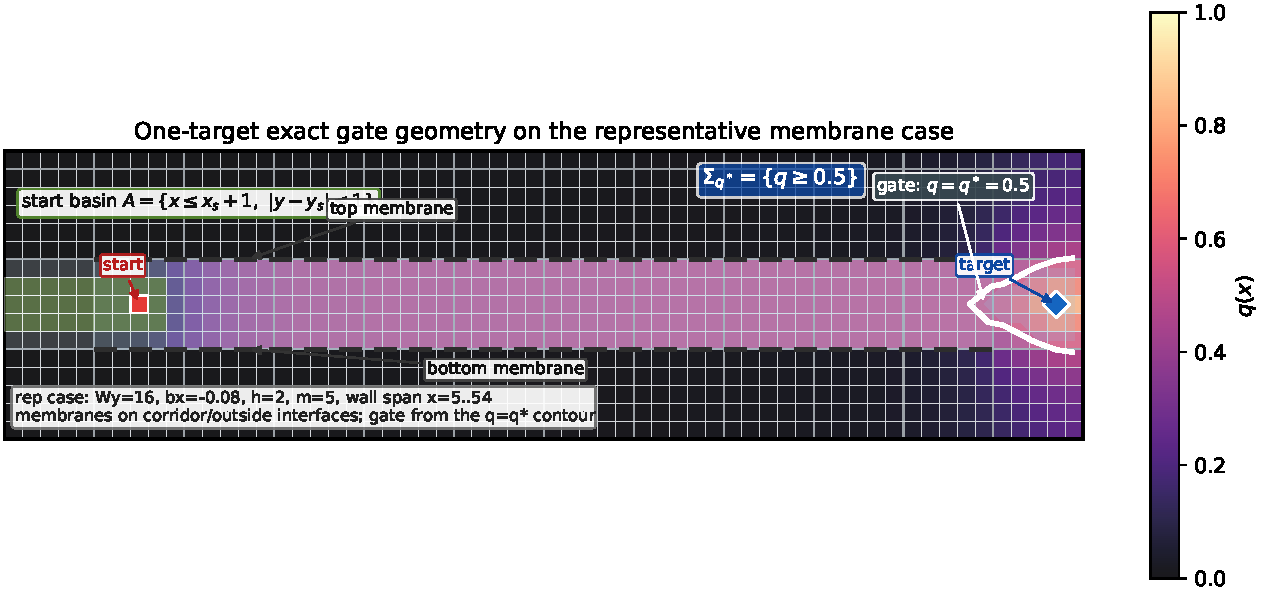
\includegraphics[width=0.86\linewidth]{../artifacts/figures/one_target_committor_control_geometry.pdf}
  \caption{Committor-based control figure for the one-target model. The $q=q^*$ contour survives, but only as an appendix control.}
\end{figure}

\end{document}
